\documentclass[12pt]{amsart}
\usepackage{amssymb,latexsym,amsmath,amsthm,enumitem,mathrsfs,geometry}
\usepackage{fullpage}
%\usepackage{showkeys}
\usepackage{fancyhdr}
\usepackage{xcolor}
\usepackage{bbm}
\usepackage{stmaryrd}
\usepackage{mathrsfs}
\usepackage{hyperref}
\usepackage{lineno}
\usepackage{diagbox}
\usepackage{array}
\usepackage{tikz}
\usetikzlibrary{arrows}
\usetikzlibrary{positioning}
\usepackage{float}
%\usepackage{pgfplots}
\usepackage{comment}
\usepackage{mathtools}
\usepackage{cleveref}
%\usepackage{refcheck}



\newtheorem{theorem}{Theorem}[section]
\newtheorem*{theorem*}{Theorem}
\newtheorem{lemma}{Lemma}[section]
\newtheorem*{remark*}{Remark}
\newtheorem{theoremletter}{Theorem}
 \newtheorem{corollary}{Corollary}[section]
\newtheorem{proposition}[theorem]{Proposition}
\newtheorem{lemmaletter}{Lemma}[section]
\renewcommand*{\thetheoremletter}{\Alph{theoremletter}}
\renewcommand*{\thelemmaletter}{\Alph{lemmaletter}}
\setcounter{lemmaletter}{1}
\newtheorem{definition}{Definition}[section]


%comment these out in final version
\newcommand{\ayla}[1]{{\color{violet}{Ayla: #1}}}
\newcommand{\terry}[1]{{\color{blue}{Terry: #1}}}
\newcommand{\eps}{\varepsilon}
\newcommand{\R}{\mathbb{R}}


\newcommand{\todo}[1]{{\color{red}{\sc(#1)}}}


\begin{document}

\numberwithin{equation}{section}

\title{On the number of exceptional intervals to the prime number theorem in short intervals}

\author[Gafni]{Ayla Gafni}
\address{Department of Mathematics, University of Mississippi, University MS 38677}
\email{argafni@olemiss.edu}
\author[Tao]{Terence Tao}
\address{Department of Mathematics, UCLA, 405 Hilgard Ave, Los Angeles CA 90024}
\email{tao@math.ucla.edu}



\keywords{}
\subjclass[2020]{}
\thanks{}


\date{\today}

\begin{abstract} For a fixed exponent $0 < \theta \leq 1$, it is expected that we have the prime number theorem in short intervals $\sum_{x \leq n < x+x^\theta} \Lambda(n) \sim x^\theta$ as $x \to \infty$.  From the recent zero density estimates of Guth and Maynard, this result is known for all $x$ for $\theta > \frac{17}{30}$ and for almost all $x$ for $\theta > \frac{2}{15}$.  Prior to this work, Bazzanella and Perelli obtained some upper bounds on the size of the exceptional set where the prime number theorem in short intervals fails.  We give an explicit relation between zero density estimates and exceptional set bounds, allowing for the most recent zero density estimates to be directly applied to give upper bounds on the exceptional set via a small amount of computer assistance.
\end{abstract}

\maketitle

\section{Introduction and background} \label{intro}

\subsection{Prime number theorem in short intervals}

The prime number theorem asserts that\footnote{See \Cref{notation-sec} for our conventions on asymptotic notation.}
$$ \sum_{n \leq x} \Lambda(n) \sim x$$
as $x \to \infty$, where $\Lambda$ is the von Mangoldt function.  Based on this, as well as random models such as the Cram\'er random model \cite{cramer}, it is natural to conjecture that the prime number theorem also holds in short intervals in the sense that
\begin{equation}\label{xyn}
 \sum_{x < n \leq x+y} \Lambda(n) \sim y
\end{equation}
as $x \to \infty$ whenever $y = x^\theta$ for a fixed $0 < \theta \leq 1$; the classical prime number theorem then corresponds to the case $\theta=1$.  An easy averaging argument (cf.  \cite[Corollary 1(i)]{bp}) shows that the difficulty of this claim increases as $\theta$ decreases, or equivalently if \eqref{xyn} holds for $\theta = \theta_0$ then it also holds for $\theta_0 \leq \theta \leq 1$.  A well-known result of Maier \cite{Maier} shows that the bound \eqref{xyn} can break down if $y$ is only of size $\log^A x$ for any fixed $A>0$, but we will not work with such small sizes of $y$ here.

It is well-known that these questions are tied to zero density theorems for the Riemann zeta function $\zeta(s)$.
For $0 \le \sigma < 1$ and $T>0$, let $\mathcal{Z}(\sigma,T)$ denote the (multi-)set
\begin{equation}
\mathcal{Z}(\sigma, T) \coloneqq  \left\{ \rho = \beta + i\gamma : \zeta(\rho)=0, \beta\ge \sigma, |\gamma|\le T \right\}
\end{equation}
of zeroes of $\zeta$ (counted with multiplicity), and let $N(\sigma, T) = \#\mathcal{Z}(\sigma, T)$ be the number of such zeroes (again counting multiplicity).  For any $0 \leq \sigma < 1$, let $A(\sigma)$ denote the least exponent for which one has the zero density theorem
$$N(\sigma, T) \ll_{\sigma, \eps} T^{A(\sigma)(1-\sigma) + \eps}$$
for any $\eps>0$, or equivalently that
\begin{equation}\label{nsig-up}
  N(\sigma, T) \leq T^{A(\sigma)(1-\sigma) + o(1)}
\end{equation}
as $T \to \infty$ (holding $\sigma$ fixed).  If $N(\sigma,T)$ vanishes for all $T$, then we adopt the convention that $A(\sigma)=-\infty$.

For $0 \leq \sigma \leq 1/2$, the Riemann--von Mangoldt formula together with the functional equation give $N(\sigma,T) \asymp T \log T$ for all large $T$, hence
\begin{equation}\label{asig-small}
A(\sigma) = \frac{1}{1-\sigma}
\end{equation}
in this regime.  For $1/2 < \sigma \leq 1$ the situation is not fully resolved; see \Cref{zero_density_table} and \Cref{fig:a_sigma} for the current best upper bounds on $A(\sigma)$.  The \emph{density hypothesis} asserts that $A(\sigma) \leq 2$ for all $\sigma$; this is currently only known for $0 \leq \sigma \leq 1/2$ and $25/32 < \sigma \leq 1$ \cite{bourgain-density}, although it is also known to follow from the Lindel\"of hypothesis (LH) \cite{ingham}.  The Lindel\"of hypothesis also implies that $A(\sigma) \leq 0$ for $3/4 < \sigma \leq 1$ \cite{halasz}.  Finally, the Riemann hypothesis of course implies that $A(\sigma)=-\infty$ for all $1/2 < \sigma < 1$.  We also make the trivial observation that $A(\sigma) (1-\sigma)$ is non-increasing in $\sigma$.

\begin{figure}
  \centering
  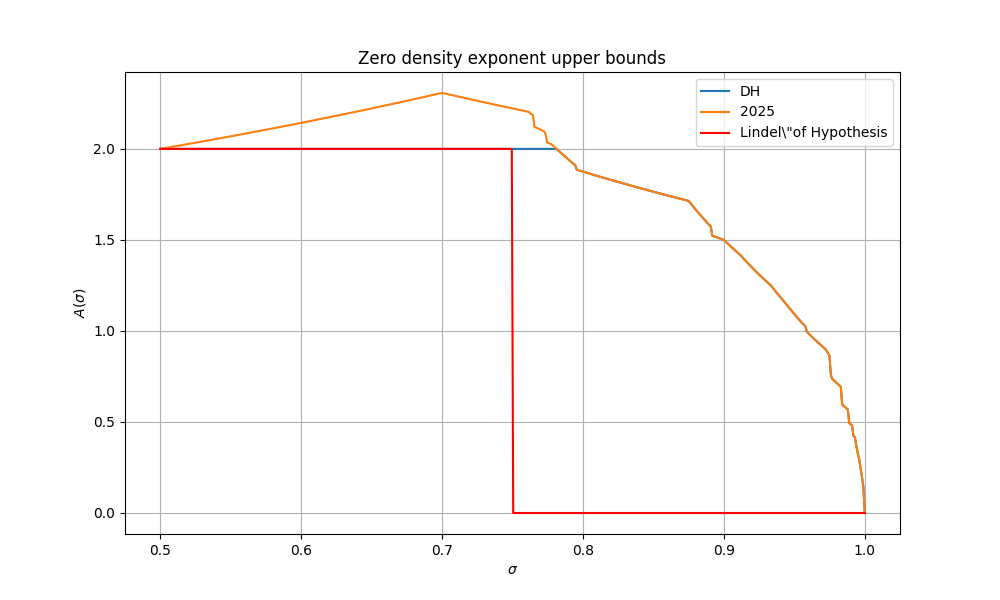
\includegraphics[width=0.8\textwidth]{a_sigma.png}
  \caption{Current best upper bounds on $A(\sigma)$ unconditionally; assuming DH; and assuming LH. 
  }\label{fig:a_sigma}
  \end{figure}


\begin{table}[ht]
\def\arraystretch{1.2}
    \centering
    \small
    \begin{tabular}{|c|c|c|}
    \hline
    $A(\sigma)$ bound & Range & Reference\\
    \hline
    $\dfrac{3}{2 - \sigma}$ & $\dfrac{1}{2} \leq \sigma \le \dfrac{7}{10} = 0.7$ & Ingham \cite{ingham} \\
    \hline
    $\dfrac{15}{3+5\sigma}$ & $\dfrac{7}{10} \leq \sigma < \dfrac{19}{25} = 0.76$ & Guth--Maynard \cite{GuthMaynard}\\
    \hline
    $\dfrac{9}{8\sigma - 2}$ & $\dfrac{19}{25} \leq \sigma < \dfrac{127}{167} = 0.7604\ldots$ & Ivic \cite{ivic} \\
    \hline
    $\dfrac{15}{13\sigma - 3}$ & $\dfrac{127}{167} \leq \sigma < \dfrac{13}{17} = 0.7647\ldots$ & Ivic \cite{ivic}\\
    \hline
    $\dfrac{6}{5\sigma - 1}$ & $\dfrac{13}{17} \leq \sigma < \dfrac{17}{22} = 0.7727\ldots$ & Ivic \cite{ivic}\\
    \hline
    $\dfrac{2}{9\sigma - 6}$ & $\dfrac{17}{22} \leq \sigma < \dfrac{41}{53} = 0.7735\ldots$ & Tao--Trudgian--Yang \cite{tty}\\
    \hline
    $\dfrac{9}{7\sigma - 1}$ & $\dfrac{41}{53} \leq \sigma < \dfrac{7}{9} = 0.7777\ldots$ & Ivic \cite{ivic}\\
    \hline
    $\dfrac{9}{8(2\sigma-1)}$ & $\dfrac{7}{9} \le \sigma < \dfrac{1867}{2347} = 0.7954\ldots$ & Tao--Trudgian--Yang \cite{tty} \\
    \hline
    $\dfrac{3}{2\sigma}$ & $\dfrac{1867}{2347} \le \sigma < \dfrac{4}{5} = 0.8$ & Bourgain \cite{bourgain} \\
    \hline
    $\dfrac{3}{2\sigma}$ & $\dfrac{4}{5} \le \sigma < \dfrac{7}{8} = 0.875$ & Ivic \cite{ivic} \\
    \hline
    $\dfrac{3}{10\sigma - 7}$ & $\dfrac{7}{8} \le \sigma < \dfrac{279}{314} = 0.8885\ldots$ & Heath--Brown \cite{HB-2} \\
    \hline
    $\dfrac{24}{30\sigma - 11}$ & $\dfrac{279}{314} \le \sigma < \dfrac{155}{174} = 0.8908\ldots$ & CDV \cite{cdv} \\
    \hline
    $\dfrac{24}{30\sigma - 11}$& $\dfrac{155}{174} \le \sigma \le \dfrac{9}{10} = 0.9$ & Ivic \cite{ivic}\\
    \hline
    $\dfrac{3}{10\sigma - 7}$ & $\dfrac{9}{10} < \sigma \le \dfrac{31}{34} = 0.9117\ldots$ & Tao--Trudgian--Yang \cite{tty}\\
    \hline
    $\dfrac{11}{48\sigma - 36}$ & $\dfrac{31}{34} < \sigma < \dfrac{14}{15} = 0.9333\ldots$ & Tao--Trudgian--Yang \cite{tty}\\
    \hline
    $\dfrac{391}{2493\sigma - 2014}$ & $\dfrac{14}{15} \le \sigma < \dfrac{2841}{3016} = 0.9419\ldots$ & Tao--Trudgian--Yang \cite{tty}\\
    \hline
    $\dfrac{22232}{163248\sigma - 134765}$ & $\dfrac{2841}{3016} \le \sigma < \dfrac{859}{908} = 0.9460\ldots$ & Tao--Trudgian--Yang \cite{tty}\\
    \hline
    $\dfrac{356}{2742\sigma - 2279}$ & $\dfrac{859}{908} \le \sigma < \dfrac{23}{24} = 0.9583\ldots$ & Tao--Trudgian--Yang \cite{tty}\\
    \hline
    $\dfrac{3}{24\sigma - 20}$ & $\dfrac{23}{24} \leq \sigma < \dfrac{2211487}{2274732} = 0.9721\ldots$ & Pintz \cite{pintz} \\
    \hline
    $\dfrac{86152}{1447460\sigma - 1311509}$ & $\dfrac{2211487}{2274732} \le \sigma < \dfrac{39}{40} = 0.975$ & Tao--Trudgian--Yang \cite{tty} \\
    \hline
    $\dfrac{2}{15\sigma - 12}$ & $\dfrac{39}{40} \leq \sigma < \dfrac{41}{42} = 0.9761\ldots$ & Pintz \cite{pintz} \\
    \hline
    $\dfrac{3}{40 \sigma - 35}$ & $\dfrac{41}{42} \leq \sigma < \dfrac{59}{60} = 0.9833\ldots$ & Pintz \cite{pintz} \\
    \hline
    $\dfrac{3}{n(1 - 2(n - 1)(1 - \sigma))}$ & \begin{tabular}{@{}c@{}}$1 - \dfrac{1}{2n(n - 1)} \le \sigma < 1 - \dfrac{1}{2n(n + 1)}$\\(for integer $n \ge 6$)\end{tabular} & Pintz \cite{pintz} \\
    \hline
    \end{tabular}
    \caption{Current best upper bounds on $A(\sigma)$, taken from the ANTEDB \cite{antedb}.}  \label{zero_density_table}

    \end{table}

The following result is standard (see, e.g., \cite[\S 13]{GuthMaynard} or \cite[Theorem 10.5, Exercise 10.5.6]{ik}), and will also be reproven here:

\begin{theorem}[Zero density theorems and PNT in short intervals]\label{folklore}  Let $A_0>0$ be such that
  \begin{equation}\label{asigma}
    A(\sigma) \leq A_0
  \end{equation}
   for all $1/2 \leq \sigma < 1$.  Let $0 < \theta < 1$ be fixed, and set $y = x^\theta$.
  \begin{itemize}
    \item[(i)] (PNT in all short intervals) If $\theta > 1-\frac{1}{A_0}$, then \eqref{xyn} holds for all $x$.
    \item[(ii)] (PNT in almost all short intervals) If $\theta > 1-\frac{2}{A_0}$, then \eqref{xyn} holds for all $x$ outside of an exceptional set of density zero.
  \end{itemize}
\end{theorem}

For instance, from \Cref{zero_density_table} one can obtain the upper bound $A(\sigma) \leq \frac{30}{13}$ for all $1/2 \leq \sigma < 1$, and hence one has the PNT in all intervals for $\theta > \frac{17}{30}$ and for almost all intervals for $\theta > \frac{2}{15}$; see \cite[Corollary 1.3, Corollary 1.4]{GuthMaynard}.  Assuming the density hypothesis, these ranges can be improved to $\theta > \frac{1}{2}$ and $\theta > 0$ respectively.

\subsection{Bounding the exceptional set}

In this paper we are interested in bounding the size of the exceptional set where \eqref{xyn} fails.  This problem was studied in \cite{baz-1}, \cite{bp}, \cite{baz-2}, and we now reproduce some notation from these papers.

\begin{definition}[Exceptional set exponent]\label{excep}\cite{bp}, \cite{baz-2}  Fix $0 < \theta < 1$.  For any $X > 1$ and $\delta > 0$, let ${\mathcal E}_\delta(X,\theta)$ denote the set of all $x \in [X,2X]$ such that
  $$ \left|\sum_{x < n \leq x+y} \Lambda(n) - y \right| \geq \delta y$$
where $y \coloneqq x^\theta$, and then let $\mu_\delta(\theta)$ denote the infimum of all exponents $\xi$ such that
$$ |{\mathcal E}_\delta(X,\theta)| \ll_{\delta,\theta} X^{\xi}$$
for all sufficiently large $X$, where $|{\mathcal E}_\delta(X,\theta)|$ denotes the Lebesgue measure of ${\mathcal E}_\delta(X,\theta)$; we adopt the convention that $\mu_\delta(\theta)=-\infty$ if ${\mathcal E}_\delta(X,\theta)$ vanishes for all sufficiently large $X$.  Finally, we set\footnote{This function $\mu(\theta)$ should not be confused with the M\"obius function, or the growth exponent for the Riemann zeta function $\zeta(\sigma+it)$ for a fixed $\sigma$.}
$$ \mu(\theta) \coloneqq \sup_{\delta > 0} \mu_\delta(\theta).$$
\end{definition}

Unpacking the definitions (setting $\delta = 1, 1/2, 1/3,\dots$ and performing a suitable diagonalization), we see that $\mu(\theta)$ is the least exponent for which the prime number theorem in short intervals \eqref{xyn} with $y = x^\theta$ holds for all $x \geq 1$ outside of an exceptional set ${\mathcal E}_\theta \subset [1,+\infty)$ with
$$ |{\mathcal E}_\theta \cap [X, 2X]| \ll X^{\mu(\theta)+o(1)}$$
as $X \to \infty$ (holding $\theta$ fixed). In particular, if $\mu(\theta) < 1$, then \eqref{xyn} would hold outside of a density zero exceptional set of parameters $x>1$.  It is easy to show that $\mu$ is a non-increasing function of $\theta$; see \cite[Corollary 1(i)]{bp}.  The exponent $\mu(\theta)$ also gives information about prime gaps: if $p_n$ denotes the $n^{\mathrm{th}}$ prime, it is easy to see that $p_{n+1}-p_n \leq 2 p_n^{\theta}$ (say) for all $n$ outside of an exceptional set ${\mathcal N}_\theta$ with\footnote{In view of results such as \cite{islam}, \cite{peck}, \cite{jarviniemi}, \cite{li}, it should be possible to improve upon \eqref{nn} by combining the methods in this paper with sieves such as the Harman sieve, but we will not attempt to do so here.}
\begin{equation}\label{nn}
   |{\mathcal N}_\theta \cap [N, 2N]| \ll N^{\mu(\theta)-\theta+o(1)}
\end{equation}
as $N \to \infty$, since any large prime gap $p_{n+1}-p_n > 2 p_n^{\theta}$ will lead to a violation of the prime number theorem \eqref{xyn} in intervals $[x,x+x^\theta]$ for $p_n \leq x \leq p_n + p_n^\theta$.

From \Cref{folklore}(i), we have $\mu(\theta) = -\infty$ for $\theta > 1 - \frac{1}{A_0}$.  It is then reasonable to expect upper bounds on $\mu(\theta)$ that are between $0$ and $1$ in the range $1-\frac{2}{A_0} < \theta \leq 1-\frac{1}{A_0}$.  In this regard, we have the following results in the literature\footnote{We thank Kaisa Matom\"aki for these and other references.}.

\begin{lemma}[Previous bounds on $\mu$]\label{baz-bound}\
  \begin{itemize}
    \item[(i)]\cite[Theorem 2(i)]{bp} For sufficiently small $\Delta>0$, we have $\mu(1/6 + \Delta) \leq 1 - c\Delta$ and $\mu(7/12-\Delta) \leq \frac{5}{8} + \frac{7}{4}\Delta + O(\Delta^2)$ for some absolute constant $c>0$.
  \item[(ii)] \cite[Theorem 2(ii)]{bp} Assuming RH, we have $\mu(\theta) \leq 1-\theta$ for $0 < \theta \leq 1/2$.
    \item[(iii)] \cite[Lemma 1]{baz-2} We have
  $$
  \mu(\theta) \leq
  \begin{cases}
  \frac{3(1-\theta)}{2} & \frac{1}{2} < \theta \leq \frac{11}{21} \\
  \frac{47-42\theta}{35}& \frac{11}{21} < \theta \leq \frac{23}{42} \\
  \frac{36\theta^2-96\theta+55}{39-36\theta} & \frac{23}{42} < \theta \leq \frac{7}{12} \\
  \end{cases}
  $$
  \end{itemize}
\end{lemma}

In \cite[Lemma 1]{baz-2}, further bounds were claimed in the region $\frac{1}{6} < \theta \leq \frac{1}{2}$, but unfortunately the argument is incomplete in that range; see \Cref{numerics-sec} for more discussion.  We also note that there is extensive literature \cite{selberg}, \cite{wolke}, \cite{cook}, \cite{huxley}, \cite{yu}, \cite{HB-1}, \cite{HB-III}, \cite{HB-2}, \cite{ivic-2}, \cite{peck}, \cite{matomaki}, \cite{HB-3}, \cite{stadlmann}, \cite{jarviniemi} on related quantities such as $\sum_{p_n \leq x} (p_{n+1}-p_n)^2$.  For instance, in \cite{selberg} it was shown that RH implies the bound $\sum_{n \leq x} (p_{n+1}-p_n)^2 \ll x \log^3 x$, which (up to $x^{o(1)}$ errors) can be recovered from \Cref{baz-bound}(ii) using \eqref{nn}.  We will not attempt to summarize the rest of this literature here, but refer the reader to \cite{antedb} instead.

The results in \Cref{baz-bound}(i) relied on the best available zero density estimates at the time, which among other things could only establish \eqref{asigma} for $A_0=12/5$.  In fact, the methods in that paper give a general relationship between $\mu$ and $A$, which is our first main result:

  \begin{theorem}[General bound]\label{gen-bound}  For any $0 < \theta < 1$, one has
\begin{equation}\label{muth}
   \mu(\theta) \leq \inf_{\eps>0} \sup_{\stackrel{0 \leq \sigma < 1}{A(\sigma) \geq \frac{1}{1-\theta}-\eps}} \mu_{2,\sigma}(\theta)
\end{equation}
where
$$ \mu_{2,\sigma}(\theta) \coloneqq (1-\theta)(1-\sigma) A(\sigma) + 2\sigma - 1.$$
Here we adopt the convention that the empty supremum is $-\infty$.
\end{theorem}

We remark that if $\tilde A(\sigma)$ is any upper bound for $A(\sigma)$ that depends continuously\footnote{One can also take $\tilde A$ to be the left-continuous majorant $\tilde A(\sigma) \coloneqq \limsup_{\sigma' \to \sigma} A(\sigma')$, which is the version of $A(\sigma)$ that is used in \cite{tty}.} on $\sigma$, then \eqref{muth} implies the simpler upper bound
\begin{equation}\label{muth-simp}
   \mu(\theta) \leq \sup_{\stackrel{0 \leq \sigma < 1}{\tilde A(\sigma) \geq \frac{1}{1-\theta}}} \tilde \mu_{2,\sigma}(\theta)
\end{equation}
where $\tilde \mu_{2,\sigma}$ is defined as $\mu_{2,\sigma}$ but with $A(\sigma)$ replaced by $\tilde A(\sigma)$.  In practice, the known upper bounds on $A(\sigma)$ are continuous in $\sigma$, so morally speaking one can set $\eps$ to zero in the above formula.  However, it is not currently known if $A(\sigma)$ itself is continuous, so we could not rigorously drop the $\eps$ parameter from the above result.

This theorem already recovers several previously mentioned results:
\begin{itemize}
  \item For $\theta > 1-\frac{1}{A_0}$, the supremum in \eqref{muth} is empty for $\eps$ small enough, and we recover \Cref{folklore}(i).
  \item For $\theta > 1-\frac{2}{A_0}$, the quantity $\mu_{2,\sigma}(\theta)$ is bounded above by $1-c(1-\sigma)$ for some $c>0$, and $A(\sigma)$ is also known (see, e.g., \cite{turan}) to go to zero as $\sigma \to 1$, and so we can also easily recover \Cref{folklore}(ii).
  \item Assuming the Riemann hypothesis, we can restrict attention to the range $0 \leq \sigma \leq 1/2$, and then \eqref{asig-small} readily gives \Cref{baz-bound}(ii).  Unconditionally, the same argument gives the bound
 \begin{equation}\label{muth-12}
   \mu(\theta) \leq \max \left( 1-\theta, \inf_{\eps>0} \sup_{\stackrel{1/2 < \sigma < 1}{A(\sigma) \geq \frac{1}{1-\theta}-\eps}} \mu_{2,\sigma}(\theta) \right).
 \end{equation}
\end{itemize}

However, \Cref{gen-bound} is not quite strong enough to recover the previous bounds in \Cref{baz-bound}(i).  This is because the arguments in that paper also relied on additional bounds on the \emph{additive energy} of zeroes, which were implicitly\footnote{The terminology ``additive energy'' was only introduced several decades later in \cite{tao-vu}.} introduced in \cite{HB-1}, and which we now define.  For $\frac12 \le \sigma < 1$ and $T>0$, let $N^*(\sigma,T)$ be given by
$$N^*(\sigma, T) =  \#\left\{ (\rho_1, \rho_2, \rho_3, \rho_4) : \rho_j = \beta_j + i\gamma_j\in \mathcal{Z}(\sigma, T), |\gamma_1 + \gamma_2 - \gamma_3 - \gamma_4|\le1 \right\}.$$
 For any $\frac{1}{2} \leq \sigma < 1$, let $A^*(\sigma)$ denote the least exponent for which one has the zero density additive energy theorem
$$N^*(\sigma, T) \ll_{\sigma, \eps} T^{A*(\sigma)(1-\sigma) + \eps}$$
for any $\eps>0$, or equivalently that
$$N^*(\sigma, T) \leq T^{A^*(\sigma)(1-\sigma) + o(1)}$$
as $T \to \infty$ (holding $\sigma$ fixed).  For $0 \leq \sigma \leq 1/2$, it is not difficult to use the Riemann--von Mangoldt formula and the functional equation to obtain the bounds
$$ N^*(\sigma,T) \asymp T^3\log^4 T$$
and hence
$$ A^*(\sigma) = \frac{3}{1-\sigma}.$$
For $1/2 < \sigma\leq 1$, the known bounds on $A^*(\sigma)$ are summarized in \Cref{zero-density-energy-table} and \Cref{fig:astar_sigma}.  One always has the trivial bound $A^*(\sigma) \leq 3 A(\sigma)$, but in many ranges of $\sigma$, stronger bounds are known.

\begin{figure}
  \centering
  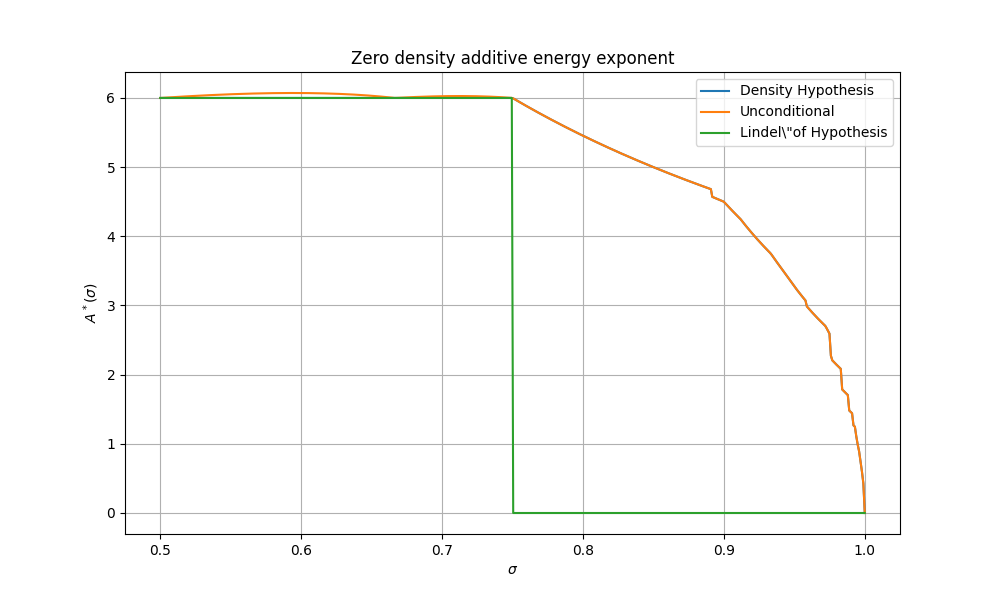
\includegraphics[width=0.8\textwidth]{astar_sigma.png}
  \caption{Current best bounds on $A^*(\sigma)$ unconditionally; assuming DH; and assuming LH.  The DH bound is the minimum of the unconditional bound and $6$, and is obscured by the other two graphs in this plot.}\label{fig:astar_sigma}
  \end{figure}

\begin{table}[ht]
    \def\arraystretch{1.2}
    \centering
\small
    \begin{tabular}{|c|c|c|}
    \hline
    $A^*(\sigma)$ bound & Range & Reference\\
    \hline
    $\dfrac{10 - 11\sigma}{(2 - \sigma)(1 - \sigma)}$ & $\dfrac{1}{2} \leq \sigma \le \dfrac{2}{3} = 0.6666\ldots$ & Heath-Brown \cite{HB-2}\\
    \hline
    $\dfrac{18 - 19\sigma}{(4 - 2\sigma)(1 - \sigma)}$ & $\dfrac{2}{3} \leq \sigma \le \dfrac{7}{10} = 0.7$ & Heath-Brown \cite{HB-2}\\
    \hline
    $\dfrac{5(18 - 19\sigma)}{2(5\sigma + 3)(1 - \sigma)}$ & $\dfrac{7}{10} \leq \sigma \le \dfrac{539 - \sqrt{42121}}{460} = 0.7255\ldots$ & Tao--Trudgian--Yang \cite{tty}\\
    \hline
    $\dfrac{2(45 - 44\sigma)}{(2\sigma + 15)(1 - \sigma)}$ & $\dfrac{539 - \sqrt{42121}}{460} \leq \sigma \le \dfrac{165}{226} = 0.7300\ldots$ & Tao--Trudgian--Yang \cite{tty}\\
    \hline
    $\dfrac{457 - 546\sigma}{2(61 - 58\sigma)(1-\sigma)}$ & $\dfrac{165}{226} \leq \sigma \le \dfrac{5831 + \sqrt{60001}}{8240} = 0.7373\ldots$ & Tao--Trudgian--Yang \cite{tty}\\
    \hline
    $\dfrac{5(18 - 19\sigma)}{2(5\sigma + 3)(1 - \sigma)}$ & $\dfrac{5831 + \sqrt{60001}}{8240} \leq \sigma \le \dfrac{42}{55} = 0.7636\ldots$ & Tao--Trudgian--Yang \cite{tty}\\
    \hline
    $\dfrac{18 - 19\sigma}{6(15\sigma - 11)(1- \sigma)}$ & $\dfrac{42}{55} \leq \sigma \le \dfrac{97}{127} = 0.7637\ldots$ & Tao--Trudgian--Yang \cite{tty}\\
    \hline
    $\dfrac{3(18-19\sigma)}{4(4\sigma-1)(1 - \sigma)}$ & $\dfrac{97}{127} \leq \sigma \le \dfrac{79}{103} = 0.7669\ldots$ & Tao--Trudgian--Yang \cite{tty}\\
    \hline
    $\dfrac{18 - 19\sigma}{2(37\sigma - 27)(1 - \sigma)}$ & $\dfrac{79}{103} \leq \sigma \le \dfrac{33}{43} = 0.7674\ldots$ & Tao--Trudgian--Yang \cite{tty}\\
    \hline
    $\dfrac{5(18 - 19\sigma)}{2(13\sigma - 3)(1 - \sigma)}$ & $\dfrac{33}{43} \leq \sigma \le \dfrac{84}{109} = 0.7706\ldots$ & Tao--Trudgian--Yang \cite{tty}\\
    \hline
    $\dfrac{18 - 19\sigma}{9(3\sigma - 2)(1 - \sigma)}$ & $\dfrac{84}{109} \leq \sigma \le \dfrac{1273 - \sqrt{128689}}{1184} = 0.7721\ldots$ & Tao--Trudgian--Yang \cite{tty}\\
    \hline
    $\dfrac{4(10 - 9\sigma)}{5(4\sigma - 1)(1 - \sigma)}$ & $\dfrac{1273 - \sqrt{128689}}{1184} \leq \sigma \le \dfrac{5}{6} = 0.8333\ldots$ & Tao--Trudgian--Yang \cite{tty}\\
    \hline
    $\dfrac{12}{4\sigma - 1}$ & $\dfrac{5}{6} \leq \sigma \le 1$ & Heath-Brown \cite{HB-2}\\
    \hline
    \end{tabular}
 
    \caption{Current best upper bounds on $A^*(\sigma)$, taken from the ANTEDB \cite{antedb}.}   \label{zero-density-energy-table}
\end{table}

We then have the following refinement of \Cref{gen-bound}:

\begin{theorem}[Refined bound]\label{refined-bound}  For any $0 < \theta < 1$, one has
$$ \mu(\theta) \leq \inf_{\eps>0} \sup_{\stackrel{0 \leq \sigma < 1}{A(\sigma) \geq \frac{1}{1-\theta}-\eps}} \min( \mu_{2,\sigma}(\theta), \mu_{4,\sigma}(\theta))$$
where
$$ \mu_{4,\sigma}(\theta) \coloneqq (1-\theta)(1-\sigma) A^*(\sigma) + 4\sigma-3.$$
\end{theorem}

As in \eqref{muth-12}, we can also bound
$$ \mu(\theta) \leq \max\left(1-\theta, \inf_{\eps>0} \sup_{\stackrel{1/2 < \sigma < 1}{A(\sigma) \geq \frac{1}{1-\theta}-\eps}} \min( \mu_{2,\sigma}(\theta), \mu_{4,\sigma}(\theta)) \right).$$

We establish \Cref{refined-bound} in \Cref{proof-sec}, following the strategy of previous works (particularly \cite{HB-2}, \cite{baz-2}) of applying the explicit formula for $\sum_{n \leq x} \Lambda(n)$, followed by $L^\infty$, $L^2$, and $L^4$ estimates for various components of that formula.

In \Cref{numerics-sec} we report on the bounds obtained by combining \Cref{refined-bound} with the estimates in \Cref{zero_density_table} and \Cref{zero-density-energy-table}.



\subsection{Acknowledgments}

AG is supported by NSF grant OIA-2229278. TT is supported by NSF grant DMS-2347850. The authors thank Kaisa Matom\"aki for providing several relevant references.


\subsection{Notation}\label{notation-sec}

We use the following asymptotic notation throughout the paper:

\begin{itemize}
\item We use $X \ll Y$, $Y \gg X$, or $X = O(Y)$ to denote the estimate $|X| \leq C Y$ for some constant $C>0$.  If we need this constant $C$ to depend on parameters, we will indicate this by subscripts, thus for instance $X \ll_\theta Y$ denotes the bound $|X| \leq C_\theta Y$ for some $C_\theta$ depending on $Y$.  We use $X \asymp Y$ to denote the estimate $X \ll Y \ll X$.
\item We use $Y = o(Z)$ as $X \to \infty$ to denote the estimate $|Y| \leq c(X) Z$ for some function $c(X)$ of a parameter $X$ that goes to zero as $X \to \infty$ (holding all other parameters fixed).  We use $Y \sim Z$ to denote the estimate $Y = (1+o(1)) Z$ as $X \to \infty$.
\end{itemize}

\section{Proof of bound}\label{proof-sec}

In this section we prove \Cref{refined-bound}, which of course implies \Cref{gen-bound} as a corollary.

We begin with some simple reductions.
Fix $0 <\theta < 1$ and $\eps$, and let $\mu$ denote the quantity
$$ \mu \coloneqq \sup_{\stackrel{0 \leq \sigma < 1}{A(\sigma) \geq \frac{1}{1-\theta}-\eps}} \min( \mu_{2,\sigma}(\theta), \mu_{4,\sigma}(\theta)),$$
thus
whenever $0 \leq \sigma < 1$ is such that $A(\sigma) \geq \frac{1}{1-\theta}-\eps$, at least one of the inequalities
\begin{equation}\label{muth-alt}
(1-\theta)(1-\sigma) A(\sigma) + 2\sigma - 1 \leq \mu
\end{equation}
and
\begin{equation}\label{muth-alt-2}
(1-\theta)(1-\sigma) A^*(\sigma) + 4\sigma - 3 \leq \mu
\end{equation}
hold. Our task is then to show that $\mu(\theta) \leq \mu$.

Fix $0 < \delta < 1$.  It will suffice to show that whenever $J$ is a natural number that is sufficiently large (depending on $\delta, \theta, \eps$), that one has the upper bound
$$|{\mathcal E}_\delta(X,\theta)| \ll_{\delta,\theta,J} X^{\mu+4/J+o(1)}$$
as $X \to \infty$ (holding the other parameters $J,\delta,\theta,\eps$ fixed).  We may of course assume that $X$ is larger than any specified absolute constant.

By subdividing $[X,2X]$ into $O_\delta(1)$ intervals of the form $[X,(1+\delta/J) X]$ and using the triangle inequality, it suffices to show that
$$\left|\left\{ X \leq x < (1+\delta/J) X: \left| \sum_{x < n \leq x + x^\theta} \Lambda(n) - x^\theta \right| \geq \delta x^\theta \right\}\right| \ll_{\delta,\theta,J} X^{\mu+4/J+o(1)}.$$
From the Brun--Titchmarsh inequality we see that for $X \leq x < (1+\delta/J) X$, one has
$$ \sum_{x < n \leq x + x^\theta} \Lambda(n) = \sum_{x < n \leq x + x/\tau} \Lambda(n) + O\left(\frac{\delta}{J} x^\theta\right)$$
where $\tau \coloneqq X^{1-\theta}$, so in particular $x/\tau = x^\theta +  O(\frac{\delta}{J} x^\theta)$.  Thus, by the triangle inequality, it will suffice (after choosing $J$ large enough) to show that
\[
\left| \left\{ X \leq x < (1+\delta/J) X : \left| \sum_{x < n \leq x + x/\tau} \Lambda(n) - \frac{x}{\tau} \right| \geq \frac{\delta}{2} \frac{X}{\tau} \right\} \right| \ll_{\delta,\theta,J,\eps} X^{\mu+4/J+o(1)}.
\]

We set $T \coloneqq J (\log^2 X) \tau = X^{1-\theta+o(1)}$.  By the explicit formula (see, e.g., \cite[Chapter 17]{davenport}) we have
$$ \sum_{x < n \leq x + x/\tau} \Lambda(n) - \frac{x}{\tau} = \sum_{\rho \in {\mathcal Z}(0,T)} \frac{(x+x/\tau)^\rho-x^\rho}{\rho} + O\left( \frac{x (\log x)^2}{T} \right).$$
By choice of $T$, the error term here is $O(\frac{1}{J} X^\theta)$.  Thus, for $J$ large enough, it suffices to show that
\begin{equation}\label{targ}
  \left|\left\{ X \leq x < (1+\delta/J) X: |S_{[0,1]}(x)| \geq \frac{\delta}{3} \frac{X}{\tau} \right\}\right| \ll_{\delta,\theta,J,\eps} X^{\mu+4/J+o(1)}
\end{equation}
where, for any subset $I$ of $[0,1]$ and any $x > 1$, we write
\begin{equation}\label{six}
   S_I(x) \coloneqq \sum_{\rho \in {\mathcal Z}(0,T): \Re \rho \in I} \frac{(x+x/\tau)^\rho-x^\rho}{\rho}.
\end{equation}

We first dispose of the region near the right edge $\sigma=1$ of the critical line.

\begin{lemma}[Contribution near the right edge]\label{right-edge}  If $\eta_0>0$ is sufficiently small depending on $\theta$, and $I \subset [1-\eta_0,1]$, then
  \begin{equation}\label{si-bound}
\sup_{X \leq x \leq 2X}|S_I(x)| \ll_\theta \exp\left(-c_\theta \frac{\log^{1/3} X}{\log\log^{1/3} X} \right)\frac{X}{\tau}
  \end{equation}
  for some $c_\theta>0$ depending only on $\theta$.
\end{lemma}

\begin{proof} This bound is essentially in \cite[\S 3]{HB-2} (with the explicit choice $\eta_0 = 10^{-7}$), but we give a proof here for the convenience of the reader.
  From the fundamental theorem of calculus and the triangle inequality, we have
\begin{align*}
\sup_{X \leq x \leq 2X}|S_I(x)| &\ll \sum_{\sigma+it \in {\mathcal Z}(1-\eta_0,T)} \frac{X}{\tau} X^{\sigma-1} \\
&\ll \frac{X}{\tau} \sum_{\sigma+it \in {\mathcal Z}(1-\eta_0,T)} X^{-\eta_0} + \int_{1-\sigma}^{\eta_0} (\log X) X^{-\eta}\ d\eta \\
&\ll \frac{X \log X}{\tau} \left( N(1-\eta_0,T) X^{-\eta_0} + \int_{0}^{\eta_0} N(1-\eta,T) X^{-\eta}\ d\eta \right)\\
&\ll \frac{X \log X}{\tau} \sup_{0 < \eta \leq \eta_0} N(1-\eta,T) X^{-\eta}.
\end{align*}
From the Vinogradov--Korobov zero-free region, we see that $N(1-\eta,T)$ vanishes unless
\begin{equation}\label{eta-vanish}
  \eta \gg_\theta \frac{1}{\log^{2/3} X \log\log^{1/3} X}.
\end{equation}
We also have the upper bound
$$ N(1-\eta,T) \ll T^{C \eta^{3/2}} \log^{O(1)} T \ll X^{C \sigma \eta^{3/2}} \log^{O(1)} X$$
for some absolute constant $C>0$; such a bound was first obtained (with $C = 12000$) in \cite[Theorem 38.2]{turan}.  The value of $C$ has improved substantially, for instance\footnote{In principle, one should be able to lower $C$ to $3\sqrt{2}$ to match the results in \cite{pintz}, but the zero density theorems there contain $T^\eps$ type losses which are unacceptable for this portion of the argument. In fact, the bounds in \cite{pintz} can be used to show that one can take $\eta_0$ to be any quantity between $0$ and $1/24$; we leave this calculation to the interested reader.} to $C=58.05$ in \cite{ford}, but the precise value of $C$ is not of importance for our purposes.  For $\eta_0$ small enough depending on $\sigma$, this then gives
$$ N(1-\eta,T) X^{-\eta} \ll X^{-\eta/2} \log^{O(1)} X$$
which, when combined with the vanishing of this expression outside of the region \eqref{eta-vanish}, gives \eqref{si-bound}.
\end{proof}

A similar argument controls intervals $I$ away from the right edge:

\begin{lemma}[$L^\infty$ bound]\label{linfty-bound}  If $I \subset [\sigma_-, \sigma_+]$ for some fixed $0 \leq \sigma_- \leq \sigma_+ \leq 1$, then
$$ \sup_{X \leq x \leq 2X} |S_I(x)| \ll_\theta X^{(1-\theta)(1-\sigma_-) A(\sigma_-) + \theta + \sigma_+ - 1 + o(1)}$$
as $X \to \infty$.
\end{lemma}

\begin{proof}
By repeating the arguments used to prove \Cref{right-edge}, we have
$$ S_I(x) \ll \frac{X \log X}{\tau} \sup_{\sigma_- \leq \sigma \leq \sigma_+} N(\sigma,T) X^{\sigma-1}.$$
If we crudely bound $N(\sigma,T) \leq N(\sigma_-,T)$ and $X^{\sigma-1} \leq X^{\sigma_+ - 1}$, we obtain
$$ S_I(x) \ll \frac{X \log X}{\tau} N(\sigma_-,T) X^{\sigma_+ - 1}.$$
The claim now follows from \eqref{nsig-up} and the definitions of $T,\tau$.
\end{proof}

We also have a second moment bound:

\begin{lemma}[$L^2$ bound]\label{l2-bound}  If $I \subset [\sigma_-, \sigma_+]$ for some fixed $0 \leq \sigma_- \leq \sigma_+ \leq 1$, then
$$ \frac{1}{X}\int_X^{2X} |S_I(x)|^2\ dx \ll_\theta X^{(1-\theta) (1-\sigma_-) A(\sigma_-) + 2\theta + 2\sigma_+ - 2 + o(1)}$$
\end{lemma}

\begin{proof}  This estimate is essentially in \cite[\S 2]{HB-2}, but for the convenience of the reader we give a proof here.  We can bound the left-hand side by
  $$ \ll \int_0^\infty |S_I(x)|^2 \psi(\log x - \log X)\ \frac{dx}{x}$$
  where $\psi$ is fixed non-negative bump function that is bounded away from zero on $[0,\log 2]$.  Using \eqref{six}, we may expand this as
$$ \sum_{\sigma+it, \sigma'+it' \in {\mathcal Z}(0,T): \sigma,\sigma' \in I} c_{\sigma+it} \overline{c}_{\sigma'+it'} X^{\sigma+\sigma'+i(t-t')} \hat \psi( t-t' - i(\sigma+\sigma'))$$
where
$$ \hat \psi(\xi) \coloneqq \int_\R \psi(u) e^{iu\xi}\ du$$
is the (complexified) Fourier transform of $\psi$, and $c_{\sigma+it}$ are the coefficients
$$ c_{\sigma+it} \coloneqq \frac{(1+1/\tau)^{\sigma+it} - 1}{\sigma+it}.$$
By standard integration by parts estimates, we have
$$ \hat \psi( t-t' - i(\sigma+\sigma')) \ll\frac{1}{(1 + |t-t'|)^{10}}$$
(say), while from the fundamental theorem of calculus one has
$$ c_{\sigma+it}, c_{\sigma'+it'} \ll \frac{1}{\tau} = X^{\theta - 1 + o(1)}.$$
By the triangle inequality, we conclude that
$$ \frac{1}{X}\int_X^{2X} |S_I(x)|^2\ dx
\ll X^{2\theta+ 2\sigma_+-2+o(1)} \sum_{\sigma+it, \sigma'+it' \in {\mathcal Z}(\sigma_-,T)} \frac{1}{(1 + |t-t'|)^{10}}.$$
From the Riemann-von Mangoldt formula, there are there are at most $O(\log T)$ zeroes $\sigma+it \in {\mathcal Z}(\sigma_-,T)$ (counting multiplicity) with $t$ in any given unit interval in $[-T,T]$, so we can bound the above expression by
$$ \ll X^{2\theta+ 2\sigma_+-2+o(1)} (\log T) N(\sigma_-, T),$$
and the claim now follows from \eqref{nsig-up} and the definitions of $T,\tau$.
\end{proof}

In a similar spirit, we have a fourth moment bound:

\begin{lemma}[$L^4$ bound]\label{l4-bound}  If $I \subset [\sigma_-, \sigma_+]$ for some fixed $0 \leq \sigma_- \leq \sigma_+ \leq 1$, then
$$ \frac{1}{X}\int_X^{2X} |S_I(x)|^4\ dx \ll_\theta X^{(1-\theta) (1-\sigma_-) A^*(\sigma_-) + 4\theta + 4\sigma_+ - 4 + o(1)}$$
\end{lemma}

\begin{proof}  Again, this estimate is essentially in \cite[\S 2]{HB-2}, but we reproduce the argument here.  With $\psi$ as before, we can bound the left-hand side by
\begin{align*}
&\ll \sum_{\sigma_1+it_1, \dots, \sigma_4+it_4 \in {\mathcal Z}(0,T): \sigma_1, \dots, \sigma_4 \in I} c_{\sigma_1+it_1} c_{\sigma_2+it_2} \overline{c}_{\sigma_3+it_3} \\
&\quad X^{\sigma_1+\sigma_2+\sigma_3+\sigma_4+i(t_1+t_2-t_3-t_4)} \hat \psi( t_1+t_2-t_3-t_4 - i(\sigma_1+\sigma_2+\sigma_3+\sigma_4))
\end{align*}
and so by using the estimates used to bound \Cref{l2-bound}, we can bound this expressin in turn by
$$ \ll X^{4\theta+4\sigma_+-4+o(1)} \sum_{\sigma_1+it_1, \dots, \sigma_4+it_4 \in {\mathcal Z}(\sigma_-,T)}
\frac{1}{(1 + |t_1+t_2-t_3-t_4|)^{10}}.$$
By a routine double counting, we can bound this expression by
$$ \ll X^{4\theta+4\sigma_+-4+o(1)} \int_\R \int_\R F(t) F(t') \frac{dt dt'}{(1+|t-t'|)^{10}}$$
where
$$ F(t) \coloneqq \# \left\{ \sigma_1+it_1, \sigma_2+it_2 \in {\mathcal Z}(\sigma_-,T) : |t_1+t_2-t| \leq \frac{1}{2} \right\}.$$
By Schur's test, this is bounded by
$$ \ll X^{4\theta+4\sigma_+-4+o(1)} \int_\R F(t)^2\ dt$$
which by expanding out the integral can be bounded by
$$ \ll X^{4\theta+4\sigma_+-4+o(1)} N^*(\sigma_-, T)$$
and the claim follows from \eqref{nsig-up} and the definitions of $T,\tau$.
\end{proof}

We can now prove \eqref{targ}.  We subdivide the interval $[0,1)$ into $J$ intervals $I$ of the form $[j/J,(j+1)/J)$ for $0 \leq j < J$.  By the pigeonhole principle (and the absence of zeroes on the line $\sigma=1$), if $|S_{[0,1]}(x)| \geq \frac{\delta}{3} \frac{X}{\tau}$, then $|S_I(x)| \geq \frac{\delta}{3J} \frac{X}{\tau}$ for one of the intervals $I$.  Thus, by the triangle inequality, it suffices to show that
\begin{equation}\label{targ-2}
 \left|\left\{ X \leq x < (1+\delta/J) X: |S_I(x)| \geq \frac{\delta}{3J} \frac{X}{\tau} \right\}\right| \ll_{\delta,\theta,J,\eps} X^{\mu+4/J+o(1)}
\end{equation}
for each such interval $I$.

Write $I = [\sigma_-,\sigma_-+1/J)$. By \Cref{right-edge}, the desired claim is true if $\sigma_- \geq 1-\eta_0$ for some sufficiently small constant $\eta_0$ (depending on $\theta$, but independent of $J$), so we may assume that $\sigma_- < 1-\eta_0$.

Suppose first that $A(\sigma_-) \leq \frac{1}{1-\theta}-\eps$.  Then we apply \Cref{linfty-bound} to conclude that
$$
\sup_{X \leq x \leq 2X}|S_I(x)|
\ll_\theta X^{- (1-\sigma_-) \eps + \theta + \frac{1}{J} + o(1)} \ll_\theta X^{-\eta_0 \eps/2 + o(1)} \frac{X}{\tau}$$
if $J$ is large enough.  Thus, for $X$ large enough, the left-hand side of \eqref{targ-2} vanishes.

It remains to consider the case when
$$ A(\sigma_-) > \frac{1}{1-\theta}-\eps.$$
By definition of $\mu$, at least one of \eqref{muth-alt}, \eqref{muth-alt-2} hold.  Suppose first that \eqref{muth-alt} holds. From \Cref{l2-bound} we have
$$ \frac{1}{X}\int_X^{2X} |S_I(x)|^2\ dx \ll_\theta X^{2\theta + \mu - 1 + 2/J + o(1)}$$
and the desired bound \eqref{targ-2} follows from the Markov inequality since $\frac{\delta}{3J} \frac{X}{\tau} =X^{2\theta+o(1)}$.
Similarly, if \eqref{muth-alt-2} holds, we have
$$ \frac{1}{X}\int_X^{2X} |S_I(x)|^4\ dx \ll_\theta X^{4\theta + \mu - 2 + 4/J + o(1)}$$
and the desired bound \eqref{targ-2} again follows from Markov's inequality as before.

\begin{remark*}
By a routine modification of the above arguments one can replace $\min(\mu_{2,\theta}, \mu_{4,\theta})$ by $\min_{1 \leq k \leq K} \mu_{2k,\theta}$ for any fixed $K$, where
$$ \mu_{2k,\sigma}(\theta) \coloneqq (1-\theta)(1-\sigma) A^{(2k)}(\sigma) + 2k\sigma-2k+1$$
and $A^{(2k)}(\sigma)$ is defined similarly to $A(\sigma)$ or $A^*(\sigma)$, but with the quantities $N(\sigma,T)$, $N^*(\sigma,T)$ replaced with the higher order additive energy
$$N^{(k)}(\sigma, T) =  \#\left\{ (\rho_1, \dots, \rho_{2k}) : \rho_j = \beta_j + i\gamma_j\in \mathcal{Z}(\sigma, T), |\gamma_1 +\dots+ \gamma_k - \gamma_{k+1} - \gamma_{2k}|\le1 \right\}.$$
The possibility of using such higher order energies in this fashion was first explored in \cite{baz-3}.  Unfortunately there are no known unconditional bounds on these energies that are not trivial consequences of existing bounds on $N(\sigma,T)$ or $N^*(\sigma,T)$.\end{remark*}

\section{Numerical calculations}\label{numerics-sec}

We now report on the bounds on $\mu(\theta)$ one obtains from \Cref{refined-bound} (or \Cref{gen-bound}) after applying various known or conjectured bounds on $A(\sigma)$.

As mentioned in the introduction, on the Riemann hypothesis (RH) we have that $\mu(\theta) \leq 1-\theta$ for $0 < \theta \leq 1/2$, and $\mu(\theta)=-\infty$ for $1/2 < \theta \leq 1$.  This appears to be the limit of what one can accomplish purely from the explicit formula.

If one only assumes the Lindel\"of hypothesis (LH), then as mentioned in the introduction, we know that $A(\sigma) \leq 2$ for $1/2 \leq \sigma \leq 3/4$ and $A(\sigma) \leq 0$ for $3/4 < \sigma < 1$.  From \eqref{muth-simp} we then have $\mu(\theta)=-\infty$ for $1/2 < \theta \leq 1$, while for $0 < \theta \leq 1/2$
 $$
   \mu(\theta) \leq \max \left( 1-\theta, \sup_{1/2 < \sigma \leq 3/4} \mu_{2,\sigma}(\theta) \right)
$$ 
and for $1/2 < \sigma \leq 3/4$ we have
$$
\mu_{2,\sigma}(\theta) \leq 2(1-\theta)(1-\sigma) + 2\sigma-1 \leq 1 - \frac{\theta}{2}
$$
and thus
$$ \mu(\theta) \leq 1 - \frac{\theta}{2}$$
for $0 < \theta \leq 1/2$.

If one just assumes the density hypothesis (DH), then we again have $\mu(\theta)=-\infty$ for $1/2 < \theta \leq 1$.  However, to get non-trivial bounds on $\mu(\theta)$ for $0 < \theta \leq 1/2$ by this method, one needs to take advantage of further zero density estimates (improving upon DH) for $\sigma$ close to one, since $\mu_{2,\sigma}(\theta)$ converges to $1$ in the limit $\sigma \to 1$.  For instance, the condition $A(\sigma) \geq \frac{1}{1-\theta}-\eps$, combined with the zero-density estimate of Pintz \cite{pintz} ensures that $\sigma \leq \frac{23}{24}$ for $\eps$ small enough, which when combined with the density hypothesis gives
$$
\mu_{2,\sigma}(\theta) \leq 2(1-\theta)(1-\sigma) + 2\sigma-1 \leq 1 - \frac{\theta}{12}
$$
and thus
$$ \mu(\theta) \leq 1 - \frac{\theta}{12}$$
for $0 < \theta \leq 1/2$.  But this bound is not optimal, due to the known improvements upon the density hypothesis for $\sigma > 25/32$, as well as bounds on the additive energy of zeroes.  The explicit evaluation of the bounds produced by \Cref{refined-bound} is complicated to state exactly, but can be performed numerically without difficulty; see \Cref{fig:conditional}.

\begin{figure}
  \centering
  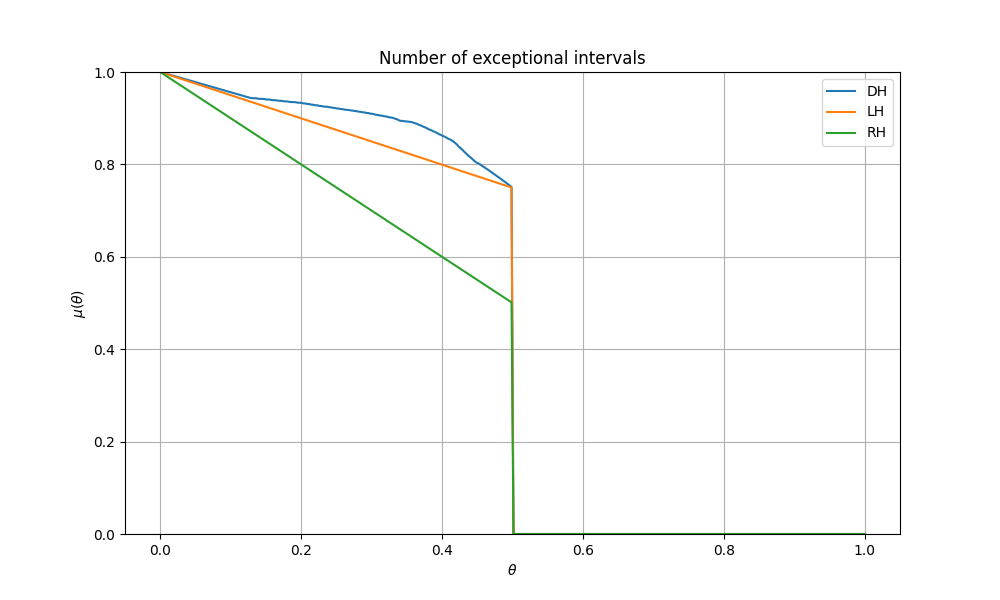
\includegraphics[width=0.8\textwidth]{conditional.png}
  \caption{Upper bounds on $\mu(\theta)$ assuming the density, Lindel\"of, and Riemann hypotheses.
  }\label{fig:conditional}
  \end{figure}

The estimates in \Cref{baz-bound}(iii) can be deduced from the the following classical estimates:
\begin{itemize}
  \item The Ingham--Huxley estimate \cite{ingham}, \cite{huxley}
$$ A(\sigma) \leq \min\left( \frac{3}{2-\sigma}, \frac{3}{3\sigma-1}\right),$$
valid for all $1/2 < \sigma < 1$;
\item The Jutila density estimate \cite{jutila} $A(\sigma) \leq 2$, valid for all $\sigma > 11/14$; and
\item The Heath-Brown estimates \cite{HB-2}, which give
$$A^*(\sigma) \leq \frac{10-11\sigma}{(2-\sigma)(1-\sigma)}$$
for $1/2 \leq \sigma \leq 2/3$,
$$A^*(\sigma) \leq \frac{18-19\sigma}{(4-2\sigma)(1-\sigma)}$$
for $2/3 < \sigma \leq 3/4$, and
$$A^*(\sigma) \leq \frac{12}{4\sigma-1}$$
for $3/4 < \sigma < 1$.
\end{itemize}

For instance, in the range $\frac{1}{2} \leq \theta \leq \frac{11}{21}$, the Jutila estimate and the condition $A(\sigma) \geq \frac{1}{1-\theta}-\eps$ then restricts one to the range $\sigma \leq \frac{11}{14}$.  Here, one can use the Heath-Brown estimates and some calculation to obtain the bound
$$ \mu_{4,\sigma}(\theta) \leq \mu_{4,3/4}(\theta) = \frac{3(1-\theta)}{2},$$
giving the first part of \Cref{baz-bound}(iii); the other two cases are treated by a similar, but more complicated, analysis.

In \cite{baz-2} it was also claimed that these methods give the bounds
$$ \mu(\theta) \leq \frac{11-6\theta}{10}$$
for $\frac{1}{6} < \theta \leq \frac{121}{173}$ and
$$ \mu(\theta) \leq \frac{3(1-\theta)}{2}$$
for $\frac{121}{173} \leq \theta \leq \frac{1}{2}$.  Unfortunately, we were not able to replicate these results.  In our language, the problem is that the Jutila density estimate no longer permits one to restrict to the range $\sigma \leq \frac{11}{14}$ when $\theta < 1/2$.  In \cite{baz-2}, the corresponding issue is with  the bound in \cite[(13)]{baz-2}: if one takes for instance $\sigma = \frac{11}{14}+2\eps$ and applies \cite[(12)]{baz-2}, one needs $X^{\theta-1+\sigma} T^{2(1-\sigma)}$ to be significantly less than $X^\theta$, but as $T$ is essentially $X^{1-\theta}$, this is only true for $\theta > 1/2$.  This issue will also restrict the range of $\alpha$ for which the proofs of \cite[Theorems 1,2]{baz-2} are complete.

By a straightforward\footnote{Code for this calculation will be uploaded to \cite{antedb}.} computer calculation (discretizing $\sigma$, $\theta$ to a finite range) one can numerically compute the bound on $\mu(\theta)$ obtained from \Cref{refined-bound} combined with \Cref{zero_density_table} and \Cref{zero-density-energy-table}; see \Cref{fig:unconditional}.  Interestingly, for a significant range of $\theta$, these bounds would not be improved under the assumption of the density hypothesis.  One could in principle give exact formulae for these bounds, but they are not particularly enlightening (and will likely be superseded as additional zero density estimates are proven).  We content ourselves with two sample calculations:
\begin{itemize}
  \item If $\theta=1-1/A_0 = 17/30$ for $A_0 = 30/13$, then the condition $A(\sigma) \geq \frac{1}{1-\theta}-\eps$ (together with the Ingham and Guth--Maynard zero density estimates) places $\sigma$ arbitrarily close to $7/10$, and then by the Heath--Brown estimates we have $A^*(\theta)$ arbitrarily close to $235/39$, and then $\mu_{4,\sigma}(\theta)$ is arbitrarily close to $7/12$; thus
  $$ \mu(17/30) \leq 7/12.$$
 \item If $\theta=1-2/A_0+\Delta = 2/15+\Delta$ for $A_0=30/13$ and $\Delta > 0$ is sufficiently small, then the condition $A(\sigma) \geq \frac{1}{1-\theta}-\eps$ restricts $\sigma$ to be bounded away from $1$ (for instance one can take $\sigma \leq 23/24$).  A routine calculation then shows that
 $$ \mu_{2,\sigma}(\theta) \leq \mu_{2,7/10}(\theta) = 1 - \frac{9}{13} \Delta$$
 and thus
 $$ \mu(2/15+\Delta) \leq 1 - \frac{9}{13} \Delta.$$ 
\end{itemize}



\begin{figure}
  \centering
  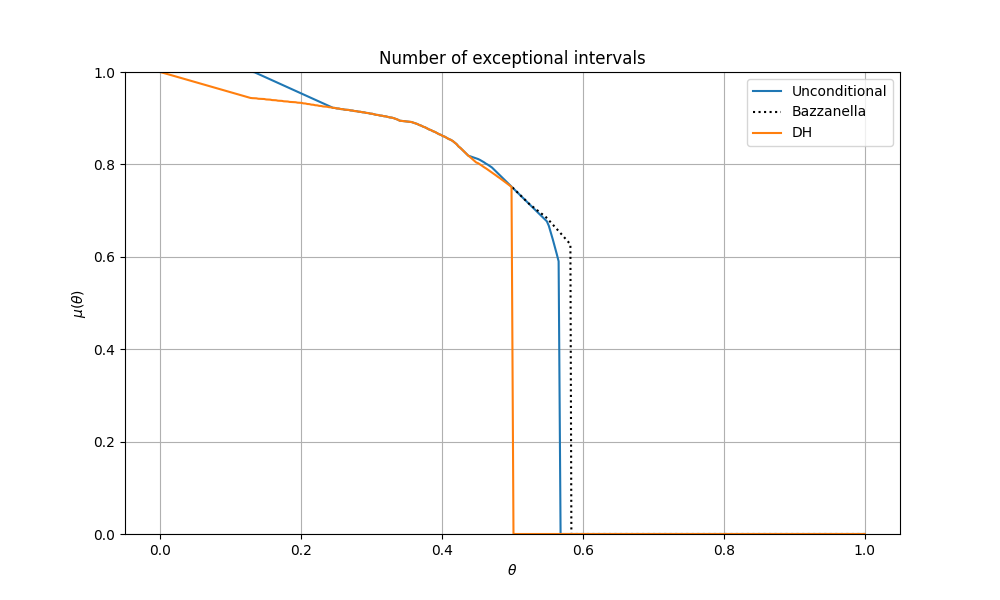
\includegraphics[width=0.8\textwidth]{unconditional.png}
  \caption{Best known unconditional bounds on $\mu(\theta)$, compared against the prior bounds of Bazzanella (for $\theta \geq 1/2$), as well as the stronger bounds assuming the density hypothesis.
  }\label{fig:unconditional}
  \end{figure}


\bibliographystyle{amsplain}

\begin{thebibliography}{10}

\bibitem{bourgain}
J. Bourgain, \emph{On the distribution of Dirichlet sums. II}, In Number theory for the millennium, I (Urbana, IL, 2000), pages 87--109. A K Peters, Natick, MA, 2002.

\bibitem{bourgain-density}
J. Bourgain, \emph{On large values estimates for Dirichlet polynomials and the density hypothesis for the Riemann zeta function}, Internat. Math. Res. Notices \textbf{2000} (2000), no. 3, 133--146.

\bibitem{baz-1}
D. Bazzanella, \emph{Primes in almost all short intervals}, Boll. Un. Mat. Ital. \textbf{7} (1995), 233--249.

\bibitem{baz-2}
D. Bazzanella, \emph{Primes in almost all short intervals II}, Boll. Unione Mat. Ital. Sez. B Artic. Ric. Mat. (8) \textbf{3} (2000), 717--726.

\bibitem{baz-3}
D. Bazzanella, \emph{Two conditional results about primes in short intervals}, Int. J. Number Theory \textbf{7} (2011), 1753--1759.

\bibitem{bp}
D. Bazzanella, A. Perelli, \emph{The exceptional set for the number of primes in short intervals}, J. Number Theory \textbf{80} (2000), 109--124.

\bibitem{cdv}
B. Chen, G. Debruyne, J. Vindas, \emph{On the density hypothesis for L-functions associated with holomorphic cusp forms}, Revista Matem\'atica Iberoamericana (2024), 1--40.

\bibitem{cook}
R. J. Cook, \emph{On the occurrence of large gaps between prime numbers}, Glasgow Math. J. \textbf{20} (1979), 43--48.

\bibitem{cramer}
H. Cram\'er, \emph{On the order of magnitude of the difference between consecutive prime numbers}, Acta Arithmetica \textbf{2} (1936), 23--46.

\bibitem{davenport}
H. Davenport, \emph{Multiplicative number theory}, 2nd ed., Springer-Verlag, New York/Berlin, 1980.

\bibitem{ford}
K. Ford, \emph{Vinogradov's integral and bounds for the Riemann zeta function}, Proc. London Math. Soc. (3) \textbf{85} (2002), 565--633.

\bibitem{GuthMaynard}
L. Guth, J. Maynard, \emph{New large value estimates for Dirichlet polynomials}, arXiv:2405.20552 [math.NT] (2024).

\bibitem{halasz}
G. Hal\'asz, P. Tur\'an, \emph{On the distribution of roots of Riemann zeta and allied functions, I}, J. Number Theory \textbf{1} (1969), 121--137.

\bibitem{HB-1}
D. R. Heath-Brown, \emph{The difference between consecutive primes, II}, J. London Math. Soc. (2) \textbf{19} (1979), 207--220.

\bibitem{HB-III}
D. R. Heath-Brown, \emph{The differences between consecutive primes, III}, J. London Math. Soc. (2) \textbf{20} (1979), 177--178.

\bibitem{HB-2}
D. R. Heath-Brown, \emph{Zero density estimates for the Riemann zeta-function and Dirichlet L-functions}, J. London Math. Soc. (2) \textbf{19} (1979), 221--232.

\bibitem{HB-3}
D. R. Heath-Brown, \emph{The number of primes in a short interval}, J. Reine Angew. Math. \textbf{389} (1988), 22--63.

\bibitem{HB-4}
D. R. Heath-Brown, \emph{The differences between consecutive primes, V}, Int. Math. Res. Not. \textbf{2021} (2021), 17514--17562.

\bibitem{huxley}
M. N. Huxley, \emph{A note on large gaps between prime numbers}, Acta Arithmetica \textbf{38} (1980), 63--68.

\bibitem{ingham}
A. E. Ingham, \emph{On the estimation of $N(\sigma,T)$}, The Quarterly Journal of Mathematics, os-11 (1) (1940), 201--202.

\bibitem{islam}
A. Islam, \emph{Multiplicative properties of integers in short intervals}, PhD thesis, Royal Holloway, University of London, 2015.

\bibitem{ivic-2}
A. Ivi\'c, \emph{On sums of large differences between consecutive primes}, Math. Ann. \textbf{241} (1979), 1--9.

\bibitem{ivic}
A. Ivi\'c, \emph{Exponent pairs and the zeta function of Riemann}, Studia Sci. Math. Hungar., \textbf{15} (1980), 157--181.

\bibitem{ik}
H. Iwaniec, E. Kowalski, \emph{Analytic number theory}, American Mathematical Society Colloquium Publications, 53. American Mathematical Society, Providence, RI, 2004.

\bibitem{jarviniemi}
O. J\"arviniemi, \emph{On large differences between consecutive primes}, arXiv:2212.10965 [math.NT] (2022).

\bibitem{jutila}
M. Jutila, \emph{Zero-density estimates for L-functions}, Acta Arithmetica \textbf{32} (1977), 52--62.

\bibitem{li}
R. Li, \emph{Primes in almost all short intervals}, arXiv:2407.05651 [math.NT] (2024).

\bibitem{Maier}
H. Maier, \emph{Primes in short intervals}, Michigan Math. J. \textbf{32} (1985), 221--225.

\bibitem{matomaki}
K. Matom\"aki, \emph{Large differences between consecutive primes}, The Quarterly Journal of Mathematics \textbf{58} (2007), 489--518.

\bibitem{peck}
A. S. Peck, \emph{On the differences between consecutive primes}, PhD thesis, University of Oxford, 1996.

\bibitem{pintz}
J. Pintz, \emph{Density theorems for Riemann’s zeta-function near the line}, Acta Arithmetica \textbf{208} (2023), 1--13.

\bibitem{selberg}
A. Selberg, \emph{On the normal density of primes in small intervals, and the difference between consecutive primes}, Arch. Math. Naturvid., \textbf{47} (1943), no. 6, 87--105.

\bibitem{stadlmann}
J. Stadlmann, \emph{On the mean square gap between primes}, arXiv:2212.10867 [math.NT] (2022).

\bibitem{antedb}
T. Tao, T. Trudgian, A. Yang, \emph{The Analytic Number Theory Exponent Database}, \url{https://github.com/teorth/expdb}

\bibitem{tty}
T. Tao, T. Trudgian, A. Yang, \emph{New exponent pairs, zero density estimates, and zero additive energy estimates: a systematic approach}, arXiv:2405.20552 (2024).

\bibitem{tao-vu}
T. Tao, V. H. Vu, \emph{Additive combinatorics}, Cambridge Studies in Advanced Mathematics, 105. Cambridge University Press, Cambridge, 2010. xviii+512 pp.


\bibitem{turan}
P. Tur\'an, \emph{On a new method of analysis and its applications}, Wiley-Interscience, New York, 1984. With the assistance of G. Hal\'asz and J. Pintz, with a foreword by Vera T. S\'os.

\bibitem{wolke}
D. Wolke, \emph{Grosse Differenzen zwischen aufeinanderfolgenden Primzahlen}, Math. Ann. \textbf{218} (1975), 269--271.

\bibitem{yu}
G. Yu, \emph{The differences between consecutive primes}, Bull. London Math. Soc. \textbf{28} (1996), 242--248.

\end{thebibliography}



\end{document}



\begin{comment}

 from the Markov inequality since $\frac{\delta}{3J} \frac{X}{\tau} =X^{4\theta+o(1)}$.

\begin{equation}\label{muth-alt}
(1-\theta)(1-\sigma) A(\sigma) + 2\sigma - 1 \leq \mu
\end{equation}
and
\begin{equation}\label{muth-alt-2}
(1-\theta)(1-\sigma) A^*(\sigma) + 4\sigma - 3 \leq \mu
\end{equation}




We can refine this estimate by incorporating the additive energy of the zeros.  For $\frac12 \le \sigma < 1$ and $T>0$, let $N^*(\sigma,T)$ be given by
$$N^*(\sigma, T) =  \#\left\{ (\rho_1, \rho_2, \rho_3, \rho_4) : \rho_j = \beta_j + i\gamma_j\in \mathcal{Z}(\sigma, T), |\gamma_1 + \gamma_2 - \gamma_3 - \gamma_4|\le1 \right\}.$$


\begin{theorem} \label{Thm: mu using L4} Suppose there are functions $A(\sigma)$,  $A^*(\sigma)$ on $[\frac12, 1)$ such that for all $\varepsilon>0$ we have
$$N(\sigma, T) \ll_{\sigma, \varepsilon} T^{A(\sigma)(1-\sigma) + \varepsilon} \quad \mbox{ and } \quad
N^*(\sigma, T) \ll_{\sigma, \varepsilon} T^{A^*(\sigma)(1-\sigma) + \varepsilon}$$
Then for $0< \theta < 1$,  we have
\begin{equation}
\mu(\theta) \le \sup_{\{\sigma: A(\sigma)\ge \frac{1}{1-\theta}\}} \left(\min\left\{  \left( (1-\theta)(1-\sigma)A(\sigma)+2\sigma -1\right), \left( (1-\theta)(1-\sigma)A^*(\sigma)+4\sigma -3 \right)\right\}\right).
\end{equation}
\end{theorem}


\section{Proof of Theorem \ref{Thm: mu using L2}}

Fix $\eta>0$, $T= X^{1-\theta}$, and let $y\in [X^{\theta + \eta}, X]$.  By the explicit formula, we have
\begin{align}\label{full sum explicit}
 \sum_{x\le n < x+y} \Lambda (n) - y  & = \sum_{\rho}\frac{(x+y)^\rho - x^\rho}{\rho}  + O\left(\frac{x (\log x)^2}{T}\right) \\
 & = \sum_{\rho}\frac{(x+y)^\rho - x^\rho}{\rho}  + O_\eta\left( y X^{-\eta} \right)  \nonumber
 \end{align}
where the sum is taken over $\rho = \beta + i\gamma$ such that $\zeta(\rho)=0$, $\beta\ge \frac12$, and $|\gamma| \le T$.
We divide the sum on the righthand side of \eqref{full sum explicit} into pieces based on ranges of $\beta$ and $\gamma$. For $\mathcal R \subset [\frac12, 1)$;  $0\le T_1<T_2$; $x\in[X,2X]$; and $y\le x$, define
\begin{equation}
\mathcal Z( \mathcal R, (T_1, T_2] ) : = \{ \rho = \beta + i\gamma : \zeta(\rho) = 0, \beta \in \mathcal R, T_1 < |\gamma| \le T_2\}.
 \end{equation}
and
\begin{equation}
S(\mathcal R; (T_1, T_2];  x, y) := \sum_{\substack{\rho = \mathcal Z( \mathcal R, (T_1, T_2] ) }}\frac{(x+y)^\rho - x^\rho}{\rho}.
\end{equation}

We want to separate the values of $\beta$ based on whether an $L^2$ or an $L^\infty$ estimate would be more beneficial.  As the bound on $N(\sigma, T)$ might not be uniform in $\sigma$, we restrict ourselves to finitely many slices.  Let $J = 2\lfloor\frac{1}{\eta}\rfloor$, and define
\begin{align}
\mathcal J_\infty  & = \left\{ \frac{J}{2}\le j \le J-2 : A(\sigma) < \frac{1}{1-\theta} \forall \sigma \in [\frac{j}{J}, \frac{j+1}{J}]\right\} \\
\mathcal J_2  & = \left\{ \frac{J}{2}\le j \le J-2 : j\not\in \mathcal J_\infty\right\} .
\end{align}
Let
\begin{equation}
\mathcal R_\infty = \bigcup_{j\in\mathcal J_\infty} [\frac{j}{J}, \frac{j+1}{J}), \quad \mathcal R_2 = \bigcup_{j\in\mathcal J_2} [\frac{j}{J}, \frac{j+1}{J}).
\end{equation}
  We have
\begin{align}
|\mathcal E_{3\delta}(X, y) | & \ll  \bigg|  \bigg\{ x\in [X,2X] : |S(\mathcal R_2; (0, T];  x, y) |  \ge \delta y\bigg \} \bigg| \nonumber
  \\ &+ \bigg|  \bigg\{ x\in [X,2X] : |S(\mathcal R_\infty; (0, T];  x, y) |  \ge \delta y\bigg \} \bigg| \nonumber
  \\ &   + \bigg|  \bigg\{ x\in [X,2X] : |S( [\frac{J-1}{J}, 1); (0, T];  x, y) |  \ge \delta y\bigg \} \bigg| .
  \label{L2 E div}
\end{align}
\todo{Insert some classical results that show the contribution from $[\frac{J-1}{J}, 1)$ is empty.}

We now consider the contribution from $\mathcal R_\infty$.  Since $\bigcup_{j\in\mathcal J_\infty} [\frac{j}{J}, \frac{j+1}{J}]$ is a compact set containing $\mathcal R_\infty$ and $A(\sigma)< \frac{1}{1-\theta}$ for all $\sigma \in   \bigcup_{j\in\mathcal J_\infty} [\frac{j}{J}, \frac{j+1}{J}]$, we can define $A:= \frac{1}{1-\theta} - \sup_{\alpha\le\sigma \le 1} A(\sigma)>0$. Then for $0<\varepsilon< \frac{A\eta}{2}$, we have
\begin{align} \nonumber
S(\alpha, 1; 0, T;  x, y) &   =   \sum_{\rho \in \mathcal Z(\mathcal R_\infty; (0, T])}\frac{(x+y)^\rho - x^\rho}{\rho}
 =  \sum_{\rho \in \mathcal Z(\mathcal R_\infty; (0, T])}\int_x^{x+y}t^{\rho-1}\, dt
 \ll y \sum_{\rho \in \mathcal Z(\mathcal R_\infty; (0, T])}x^{\beta-1}  \\   \nonumber
 & \ll y \int_{\frac12}^{\frac{J-1}{J}} x^{\sigma - 1}\mathbbm{1}_{\mathcal R_\infty} (\sigma)\, dN(\sigma, T) \ll_{\varepsilon} y(\log T) T^\varepsilon \int_{\frac12}^{\frac{J-1}{J}}\left(\frac{T^{A(\sigma)}}{x}\right)^{1- \sigma}d\sigma \\  \nonumber
 & \ll_\varepsilon y(\log T)   \int_{\frac12}^{\frac{J-1}{J}} T^{- A (1- \sigma) + \varepsilon}d\sigma
 \\ &  \ll_\eta y T^{-A\eta/2}.\label{L infinity bound}
  \end{align}
Thus we have,
\begin{equation} \label{L-infty gives null}
\bigg\{ x\in [X,2X] : |S(\alpha, 1; 0, T;  x, y) |  \ge \delta y\bigg \} = \varnothing.
\end{equation}
\todo{Maybe add a sentence explaining that the above argument is uniform in $\delta$... or fix it if it isn't}

We now use $L^2$ estimates to study the contribution from $\mathcal R_2$.  For $M\ge \log X$, Heath-Brown \todo{citation, Lemma 1} gives
\begin{equation}\label{eq: HB L2}
\int_X^{2X}\left|S\left([\frac mM, \frac{m+1}M); (3^{n-1}, 3^n]; x, \frac{x}{\tau}\right)\right|^2 dx  \ll X^{1+ 2m/M} \min(\tau^{-1}, 3^{-n})^2 M^2 N(\frac mM, 3^{n}).
\end{equation}
This bound is uniform in $m, n, x, \tau$, and $X$ provided that $1\le \tau \le X$ and $2\le X \le x \le 2X$.  However, the input bound on $N(\sigma, T)$ may not be uniform in $\sigma$.  Thus, we divide the interval $[1/2, 1)$ into $\log X$ slices to apply \eqref{eq: HB L2}, then combine those slices into $J= 2\lfloor\frac{1}{\varepsilon}\rfloor$ slabs.  Since $J$ is bounded independently of $X$, we can safely use the $N(\sigma, T)$ bound.  If $\frac{m}{M} \in [\frac{j}{J}, \frac{j+1}{J})$ then
$$ X^{1+ 2m/M} \min(\tau^{-1}, 3^{-n})^2 M^2 N(\frac mM, 3^{n}) \le  X^{1+ 2(j+1)/J} \min(\tau^{-1}, 3^{-n})^2 M^2 N(\frac jJ, 3^{n}). $$
 Moreover, there are at most $\eta M + 1$  $m$-slices in each $j$-slab.

 By the triangle inequality, we have
\begin{align}
\int_X^{2X}\left|S( \mathcal R_2; (3^{n-1}, 3^n];   x, \frac{x}{\tau}) \right| ^2 dx & \le \left(\sum _{\substack{\frac{M}{2} \le m <  M\\ \frac{m}{M}\in \mathcal R_2}} \left(\int_X^{2X} \left|S\left([\frac mM, \frac{m+1}M); (3^{n-1}, 3^n]; x, \frac{x}{\tau}\right)\right|^2 dx\right)^{\frac12}\right)^2 \\
& \ll \min(\tau^{-1}, 3^{-n})^2 X M^2 \left(\sum _{\substack{\frac{M}{2} \le m <  M\\ \frac{m}{M}\in \mathcal R_2}} X^{\frac mM} N(\frac mM, 3^n)^{\frac12}\right)^2 \\
& \ll_{\varepsilon} \min(\tau^{-1}, 3^{-n})^2 X^{1+\eta} M^3  \left(\sum _{\substack{\frac{J}{2} \le j <  J\\ j\in\mathcal J_2}} X^{\frac jJ} N(\frac jJ, 3^n)^{\frac12}\right)^2 \\
%& \le  \min(\tau^{-1}, 3^{-n})^2 X^{1+\eta} M^5 \left(\max_{\frac{J}{2} \le j < \alpha J} X^{\frac jJ} N( \frac jJ, 3^n)^{\frac12}\right)^2 \\
& \le \min(\tau^{-1}, 3^{-n})^2 X^{1+\eta} M^5 \max_{\substack{\frac{J}{2} \le j <  J\\ j\in\mathcal J_2}} X^{2\frac jJ} N( \frac jJ, 3^n) .
\end{align}
Summing over $n$ such that $3^n \le T$, we have
\begin{align}
\int_X^{2X} \left|S(\mathcal R_2;( 0, T];   x, \frac{x}{\tau}) \right| ^2 dx & \le  \left(\sum _{3^n \le T} \left(\int_X^{2X} \left|S\left( \mathcal R_2; (3^{n-1}, 3^n]; x, \frac{x}{\tau}\right)\right|^2 dx\right)^{\frac12}\right)^2 \\
& \ll_{\varepsilon}    X^{1+\eta} M^5 \left(\sum _{3^n \le T} \min(\tau^{-1}, 3^{-n})\right )^2 \max_{\substack{\frac{J}{2} \le j <  J\\ j\in\mathcal J_2}} X^{2\frac jJ} N( \frac jJ, T)\\
& \ll_{\varepsilon}  X^{1+\eta} M^5  \tau^{-2}(\log \tau )^2\max_{\substack{\frac{J}{2} \le j <  J\\ j\in\mathcal J_2}} X^{2\frac jJ} N( \frac jJ, T)\\
& \ll_{\varepsilon}  X^{1+\eta} (\log X)^5  \tau^{-2}(\log \tau )^2\sup_{\sigma\in \mathcal R_2} X^{2\sigma}T^{A(\sigma)(1-\sigma)+ \varepsilon}.
\end{align}


Now we choose $\tau = \frac{X}{y}$, so that $y \le \frac {x}{\tau}$ and $S(  \mathcal R; (0, T];   x, \frac{x}{\tau}) \ge S( \mathcal R; (0, T];   x, y)$. Then, recalling that the contribution from $ \mathcal R_\infty$ and $\sigma>\frac{J-1}{J}$ is empty, we have
\begin{align}
|\mathcal E_{2\delta}(X, y) | & \ll  \bigg|  \bigg\{ x\in [X,2X] : |S( \mathcal R_2; (0, T];  x, y) |  \ge \delta y\bigg \} \bigg| \\
  &  \le  \bigg|  \bigg\{ x\in [X,2X] : |S( \mathcal R_2; (0, T];  x, \frac{x}{\tau}) |  \ge \delta y\bigg \} \bigg|
 \\ & \ll  (\delta y)^{-2} \int_X^{2X} |S( \mathcal R_2; (0, T];  x, \frac{x}{\tau}) | ^2 dx
 %\\ & \ll_{\varepsilon}   \delta^{-2} (\log X)^5 (\log \tau )^2 \max _{\sigma\in \mathcal R_2} X^{2\sigma-1} N( \sigma, T)
 \\ & \ll_{\varepsilon}  \delta^{-2} (\log X)^5 (\log \tau )^2\sup_{\sigma\in \mathcal R_2} X^{2\sigma-1+ \eta}T^{A(\sigma)(1-\sigma)+ \varepsilon}
 \\ & \ll_{\varepsilon}  \delta^{-2} (\log X)^7 \sup _{\sigma\in \mathcal R_2} X^{2\sigma-1 + A(\sigma)(1-\sigma)(1-\theta)+ \varepsilon'}.
\end{align}
This bound is uniform in $y$, so we have
$$\mu(\theta) \le \sup_{\sigma\in \mathcal R_2} (1-\theta)(1-\sigma)A(\sigma)+2\sigma -1.$$

Note that our construction of $\mathcal R_2$ is dependent on $J$. However, the set $\{\sigma: A(\sigma)\ge \frac{1}{1-\theta}\}$ is equal to the infinite intersection of the sets $\mathcal R_2$ as $J\rightarrow \infty$ (or equivalently $\eta\rightarrow 0$).  Thus, we obtain the result:
$$\mu(\theta) \le \sup_{\{\sigma: A(\sigma)\ge \frac{1}{1-\theta}\}} (1-\theta)(1-\sigma)A(\sigma)+2\sigma -1.$$


\begin{comment}
\section{Proof of Theorem \ref{Thm: mu using L2 } with block intervals}

Fix $\varepsilon>0$, $T= X^{1-\theta}$, and let $y\in [X^{\theta + \varepsilon}, X]$.  By the explicit formula, we have
\begin{align}\label{full sum explicit}
 \sum_{x\le n < x+y} \Lambda (n) - y  & = \sum_{\rho}\frac{(x+y)^\rho - x^\rho}{\rho}  + O\left(\frac{x (\log x)^2}{T}\right) \\
 & = \sum_{\rho}\frac{(x+y)^\rho - x^\rho}{\rho}  + O\left( y X^{-\varepsilon} \right)  \nonumber
 \end{align}
where the sum is taken over $\rho = \beta + i\gamma$ such that $\zeta(\rho)=0$, $\beta\ge \frac12$, and $|\gamma| \le T$.
We divide the sum on the righthand side of \eqref{full sum explicit} into pieces based on ranges of $\beta$ and $\gamma$.  For $\frac12\le \sigma_1<\sigma_2\le1$; $0\le T_1<T_2$; $x\in[X,2X]$; and $y\le x$, define
\begin{equation}
S(\sigma_1, \sigma_2; T_1, T_2;  x, y) := \sum_{\substack{\rho = \beta + i\gamma \\\sigma_1\le \beta < \sigma_2 \\ T_1 < |\gamma| \le T_2}}\frac{(x+y)^\rho - x^\rho}{\rho},
\end{equation}
where, as above, the sum is taken over zeros of the Riemann zeta-function.   We have
\begin{align}
|\mathcal E_{2\delta}(X, y) | & \ll  \bigg|  \bigg\{ x\in [X,2X] : |S(1/2, \alpha; 0, T;  x, y) |  \ge \delta y\bigg \} \bigg| \nonumber
  \\ &+ \bigg|  \bigg\{ x\in [X,2X] : |S(\alpha, 1; 0, T;  x, y) |  \ge \delta y\bigg \} \bigg|. \label{L2 E div}
\end{align}


We first consider the contribution from $\beta \ge \alpha$.  Let $Z(T) = \sup \{ \sigma : \mathcal{Z}(\sigma, T)\ne \varnothing\}$.  By the zero-free region \todo{citation} there exists $c>0$ such that
$$Z(T) \le 1 - \frac{c}{(\log T)^{\frac23}(\log\log T)^{\frac13}}.$$
Let $A:= \frac{1}{1-\theta} - \sup_{\alpha\le\sigma \le 1} A(\sigma)$, which is positive by our choice of $\alpha$.  Then for $0<\epsilon< \frac A2 (1-Z(T))$, we have
\begin{align} \nonumber
S(\alpha, 1; 0, T;  x, y) &   =   \sum_{\substack{\rho = \beta + i\gamma \\ \beta \ge \alpha \\ |\gamma| \le T}}\frac{(x+y)^\rho - x^\rho}{\rho}
 =  \sum_{\substack{\rho = \beta + i\gamma \\ \beta \ge \alpha \\ |\gamma| \le T}}\int_x^{x+y}t^{\rho-1}\, dt
 \ll y \sum_{\substack{\rho = \beta + i\gamma \\ \beta  \ge \alpha \\ |\gamma| \le T}} x^{\beta-1}  \\   \nonumber
 & \ll y \int_{\alpha}^{Z(T)} x^{\sigma - 1}\, dN(\sigma, T) \ll y(\log x) T^\varepsilon \int_{\alpha}^{Z(T)} \left(\frac{T^{A(\sigma)}}{x}\right)^{1- \sigma}d\sigma \\  \nonumber
 & \ll y(\log x)   \int_{\alpha}^{Z(T)} T^{-\frac A2 (1- \sigma)}d\sigma \ll y T^\varepsilon \exp\left( - \frac{Ac(\log T)^{\frac13}}{2(\log\log T)^{\frac13}}\right)
 \\ & \ll y (\log T)^{-B} \label{large beta}
  \end{align}
for all $B$.  Thus, for each $\delta>0$, we can choose $B$ sufficiently large so that
\begin{equation} \label{L-infty gives null}
\bigg\{ x\in [X,2X] : |S(\alpha, 1; 0, T;  x, y) |  \ge \delta y\bigg \} = \varnothing.
\end{equation}

We now use $L^2$ estimates to study the contribution from $\beta < \alpha$.  For $M\ge \log X$, Heath-Brown \todo{citation, Lemma 1} gives
\begin{equation}\label{eq: HB L2}
\int_X^{2X}\left|S\left(\frac mM, \frac{m+1}M; 3^{n-1}, 3^n; x, \frac{x}{\tau}\right)\right|^2 dx  \ll X^{1+ 2m/M} \min(\tau^{-1}, 3^{-n})^2 M^2 N(\frac mM, 3^{n}).
\end{equation}
This bound is uniform in $m, n, x, \tau$, and $X$ provided that $1\le \tau \le X$ and $2\le X \le x \le 2X$.  However, the input bound on $N(\sigma, T)$ may not be uniform in $\sigma$.  Thus, we divide the interval $[1/2, 1)$ into $\log X$ slices to apply \eqref{eq: HB L2}, then combine those slices into $J= 2/\varepsilon$ slabs.  Since $J$ is bounded independently of $X$, we can safely use the $N(\sigma, T)$ bound.  If $\frac{m}{M} \in [\frac{j}{J}, {j+1}{J}]$ then
$$ X^{1+ 2m/M} \min(\tau^{-1}, 3^{-n})^2 M^2 N(\frac mM, 3^{n}) \le  X^{1+ 2(j+1)/J} \min(\tau^{-1}, 3^{-n})^2 M^2 N(\frac jJ, 3^{n}). $$
 Moreover, there are at most $\varepsilon M + 1$  $m$-slices in each $j$-slab.

 By the triangle inequality, we have
\begin{align}
\int_X^{2X}\left|S( \frac12, \alpha; 3^{n-1}, 3^n;   x, \frac{x}{\tau}) \right| ^2 dx & \le \left(\sum _{\frac{M}{2} \le m < \alpha M} \left(\int_X^{2X} \left|S\left(\frac mM, \frac{m+1}M; 3^{n-1}, 3^n; x, \frac{x}{\tau}\right)\right|^2 dx\right)^{\frac12}\right)^2 \\
& \ll \min(\tau^{-1}, 3^{-n})^2 X M^2 \left(\sum _{\frac{M}{2} \le m < \alpha M} X^{\frac mM} N(\frac mM, 3^n)^{\frac12}\right)^2 \\
& \ll_{\varepsilon} \min(\tau^{-1}, 3^{-n})^2 X^{1+\eta} M^3  \left(\sum _{\frac{J}{2} \le j < \alpha J} X^{\frac jJ} N(\frac jJ, 3^n)^{\frac12}\right)^2 \\
%& \le  \min(\tau^{-1}, 3^{-n})^2 X^{1+\eta} M^5 \left(\max_{\frac{J}{2} \le j < \alpha J} X^{\frac jJ} N( \frac jJ, 3^n)^{\frac12}\right)^2 \\
& \le \min(\tau^{-1}, 3^{-n})^2 X^{1+\eta} M^5 \max_{\frac{J}{2} \le j < \alpha J} X^{2\frac jJ} N( \frac jJ, 3^n) .
\end{align}
Summing over $n$ such that $3^n \le T$, we have
\begin{align}
\int_X^{2X} \left|S( \frac 12, \alpha; 0, T;   x, \frac{x}{\tau}) \right| ^2 dx & \le  \left(\sum _{3^n \le T} \left(\int_X^{2X} \left|S\left( \frac 12, \alpha; 3^{n-1}, 3^n; x, \frac{x}{\tau}\right)\right|^2 dx\right)^{\frac12}\right)^2 \\
& \ll_{\varepsilon}    X^{1+\eta} M^5 \left(\sum _{3^n \le T} \min(\tau^{-1}, 3^{-n})\right )^2 \max_{\frac{J}{2} \le j < \alpha J} X^{2\frac jJ} N( \frac jJ, T)\\
& \ll_{\varepsilon}  X^{1+\eta} M^5  \tau^{-2}(\log \tau )^2\max_{\frac{J}{2} \le j < \alpha J} X^{2\frac jJ} N( \frac jJ, T)\\
& \ll_{\varepsilon}  X^{1+\eta} (\log X)^5  \tau^{-2}(\log \tau )^2\sup_{\frac{1}{2} \le \sigma < \alpha} X^{2\sigma}T^{A(\sigma)(1-\sigma)+ \varepsilon}.
\end{align}


Now we choose $\tau = \frac{X}{y}$, so that $y \le \frac {x}{\tau}$ and $S( \sigma_1, \sigma_2; 0, T;   x, \frac{x}{\tau}) \ge S( \sigma_1, \sigma_2; 0, T;   x, y)$. Then, recalling that the contribution from $\beta > \alpha$ is empty, we have
\begin{align}
|\mathcal E_{2\delta}(X, y) | & \ll  \bigg|  \bigg\{ x\in [X,2X] : |S(1/2, \alpha; 0, T;  x, y) |  \ge \delta y\bigg \} \bigg| \\
  &  \le  \bigg|  \bigg\{ x\in [X,2X] : |S(1/2, \alpha; 0, T;  x, \frac{x}{\tau}) |  \ge \delta y\bigg \} \bigg|
 \\ & \ll  (\delta y)^{-2} \int_X^{2X} |S(1/2, \alpha; 0, T;  x, \frac{x}{\tau}) | ^2 dx
 %\\ & \ll_{\varepsilon}   \delta^{-2} (\log X)^5 (\log \tau )^2 \max _{\frac 12  \le \sigma < \alpha} X^{2\sigma-1} N( \sigma, T)
 \\ & \ll_{\varepsilon}  \delta^{-2} (\log X)^5 (\log \tau )^2\sup_{\frac{1}{2} \le \sigma < \alpha} X^{2\sigma-1+ \varepsilon}T^{A(\sigma)(1-\sigma)+ \varepsilon}
 \\ & \ll_{\varepsilon}  \delta^{-2} (\log X)^7 \sup _{\frac 12  \le \sigma < \alpha} X^{2\sigma-1 + A(\sigma)(1-\sigma)(1-\theta)+ \varepsilon'}.
\end{align}

This bound is uniform in $y$, so we obtain the result:
$$\mu(\theta) \le \sup_{\frac12 \le \sigma < \alpha} (1-\theta)(1-\sigma)A(\sigma)+2\sigma -1.$$




%% This is the old proof.  The new one extends to L4 in a nicer way
We now use $L^2$ estimates to study the contribution from $\beta\le \alpha$.  Letting $\Delta = X^{\theta-1}$ we have
 \begin{align}  \nonumber
 & \int_X^{2X} \bigg| \sum_{\substack{\rho = \beta + i\gamma \\\frac12 \beta \le \alpha \\ |\gamma| \le T}}\frac{(x+y)^\rho - x^\rho}{\rho} \bigg|^2 \, dx \nonumber \\
 & \ll   \int_X^{2X} \bigg|\frac{y}{\Delta X} \sum_{\substack{\rho = \beta + i\gamma \\ \beta \le \alpha \\ |\gamma| \le T}}\left(\frac{(x+\Delta x)^\rho - x^\rho}{\rho}\right)  +O(\Delta X) \bigg|^2 \, dx   \\
  & = \frac{y^2}{\Delta^2 X^2} \sum_{\rho_1, \rho_2} \left(\frac{(1+\Delta)^{\rho_1} - 1}{\rho_1}\right)\overline{\left(\frac{(1+\Delta)^{\rho_2} - 1}{\rho_2}\right)} \int_X^{2X} x^{\rho_1+\overline{\rho_2}} \, dx + O(\Delta^2X^{3}) \nonumber  \\
 & \ll  \frac{y^2}{X^2}   \sum_{\frac12 \le \beta_1, \beta_2 \le \alpha}\frac{X^{\beta_1 + \beta_2+ 1}}{|\rho_1+\overline{\rho_2}+1| }  + X^{2\theta+1}\nonumber \\
&  \ll \frac{y^2}{X^2}   \sum_{\frac12 \le \beta_1\le \alpha}X^{2 \beta_1+ 1} \sum_{\frac12 \le \beta_2\le \beta_1}|\rho_1+\overline{\rho_2}+1|^{-1} +y^2X^{1-\varepsilon}\\
& \ll y^2\left( (\log X)^2 \sup_{\frac12 \le \sigma\le \alpha} X^{2\sigma-1} N(\sigma,T) + X^{1-\varepsilon} \right) \nonumber \\
& \ll y^2 (\log X)^2 (\log T)^B \sup_{\frac12 \le \sigma\le \alpha} X^{2\sigma-1}T^{A(\sigma)(1-\sigma)} \nonumber \\
& \ll y^2\ (\log X)^2 (\log T)^B \sup_{\frac12 \le \sigma\le \alpha} X^{(1-\theta)(1-\sigma)A(\sigma)+2\sigma -1}.\label{small beta}
 \end{align}

We now combine these estimates to study the size of $\mathcal E(X, \theta)$.  Fix $\delta>0$ and $y\in [X^{\theta+\varepsilon}, X]$.  By \eqref{large beta} we see that the contribution to the sum from zeros with real part $\beta > \alpha$ is $o(y)$.  Thus, using the explicit formula and \eqref{small beta} we have
\begin{align}\nonumber
|\mathcal {\mathcal E}_\delta(X, y) | & \ll  \bigg|  \bigg\{ x\in [X,2X] : \bigg| \sum_{\substack{\rho = \beta + i\gamma \\ \frac12 \le \beta \le \alpha \\ |\gamma| \le T}}\frac{(x+y)^\rho - x^\rho}{\rho} \bigg|  \ge \delta y\bigg \} \bigg| \\ \nonumber
& \le \frac{1}{\delta^2 y^2}  \int_X^{2X} \bigg| \sum_{\substack{\rho = \beta + i\gamma \\\frac12\le \beta \le \alpha \\ |\gamma| \le T}}\frac{(x+y)^\rho - x^\rho}{\rho} \bigg|^2 \, dx \nonumber \\ \nonumber
& \ll_{\delta} (\log X)^{2+B}  \sup_{\frac12 \le \sigma\le \alpha} X^{(1-\theta)(1-\sigma)A(\sigma)+2\sigma -1}.
\end{align}
This bound is uniform in $y$, so we obtain the result:
$$\mu(\theta) \le \sup_{\frac12 \le \sigma\le \alpha} (1-\theta)(1-\sigma)A(\sigma)+2\sigma -1.$$

\section{Proof of Theorem \ref{Thm: mu using L4}}

We follow the proof of Theorem \ref{Thm: mu using L2}, but now include a third set $\mathcal R_4$, which we will study using $L^4$ estimates.
Fix $\eta>0$, let $J = 2\lfloor\frac{1}{\eta}\rfloor$, and define
\begin{align}
\mathcal J_\infty  & = \left\{ \frac{J}{2}\le j \le J-2 : A(\sigma) < \frac{1}{1-\theta} \forall \sigma \in [\frac{j}{J}, \frac{j+1}{J}]\right\}, \\
\mathcal J_4  & = \left\{ \frac{J}{2}\le j \le J-2 : j\not\in \mathcal J_\infty, A^*(\sigma) - A(\sigma) < \frac{2}{1-\theta} \forall \sigma \in [\frac{j}{J}, \frac{j+1}{J}]\right\}, \\
\mathcal J_2  & = \left\{ \frac{J}{2}\le j \le J-2 : j\not\in \mathcal J_\infty\cup  \mathcal J_4 \right\} .
\end{align}
Let
\begin{equation}
\mathcal R_\infty = \bigcup_{j\in\mathcal J_\infty} [\frac{j}{J}, \frac{j+1}{J}), \quad \mathcal R_4 = \bigcup_{j\in\mathcal J_4} [\frac{j}{J}, \frac{j+1}{J})\quad \mathcal R_2 = \bigcup_{j\in\mathcal J_2} [\frac{j}{J}, \frac{j+1}{J}).
\end{equation}
  We have
\begin{align}
|\mathcal E_{4\delta}(X, y) | & \ll  \bigg|  \bigg\{ x\in [X,2X] : |S(\mathcal R_2; (0, T];  x, y) |  \ge \delta y\bigg \} \bigg| \nonumber
 \\ &+ \bigg|  \bigg\{ x\in [X,2X] : |S(\mathcal R_4; (0, T];  x, y) |  \ge \delta y\bigg \} \bigg| \nonumber
  \\ &+ \bigg|  \bigg\{ x\in [X,2X] : |S(\mathcal R_\infty; (0, T];  x, y) |  \ge \delta y\bigg \} \bigg| \nonumber
  \\ &   + \bigg|  \bigg\{ x\in [X,2X] : |S( [\frac{J-1}{J}, 1); (0, T];  x, y) |  \ge \delta y\bigg \} \bigg| .
  \label{L4 split}
\end{align}


The analysis of the contributions from  $\mathcal R_2$, $\mathcal R_\infty$, and $\sigma>\frac{J-1}{J}$ are inherited from the previous proof.  In particular, we have

\begin{equation}  \label{R2 contribution in L4 proof}
 \bigg|  \bigg\{ x\in [X,2X] : |S(\mathcal R_2; (0, T];  x, y) |  \ge \delta y\bigg \} \bigg|
 \ll \delta^{-2} (\log X)^7 \sup _{\sigma \in \mathcal R_2} X^{2\sigma-1} T^{A(\sigma)(1-\sigma)+ \varepsilon}
 %\ll \delta^{-2} (\log X)^6 \sup _{\frac 12  \le \sigma < \alpha'} X^{2\sigma-1 + A(\sigma)(1-\sigma)(1-\theta)+ \varepsilon}.
\end{equation}
and
\begin{equation}
\bigg\{ x\in [X,2X] : |S(\alpha, 1; 0, T;  x, y) |  \ge \delta y\bigg \} \bigcup  \bigg\{ x\in [X,2X] : |S( [\frac{J-1}{J}, 1); (0, T];  x, y) |  \ge \delta y\bigg \} = \varnothing. \label{infty contr in L4 proof}
\end{equation}

It remains to consider the contribution from $\mathcal R_4$.   For $M\ge \log X$,  Heath-Brown \todo{citation, Lemma 1} also shows that
\begin{equation}
\int_X^{2X} \left|S\left([\frac mM, \frac{m+1}M); (3^{n-1}, 3^n]; x, \frac{x}{\tau}\right)\right|^4 dx  \ll X^{1+ 4m/M} \min(\tau^{-1}, 3^{-n})^4 M^4 N^*(\frac mM, 3^{n}).
\end{equation}

\begin{comment}
% Full HB Lemma... maybe don't need it
Let $M\ge \log X$.  Heath-Brown \todo{citation, Lemma 1} shows that
\begin{align}
S\left(\frac mM, \frac{m+1}M; 3^{n-1}, 3^n; x, \frac{x}{\tau}\right) &  \ll X^{m/M} \min(\tau^{-1}, 3^{-n}) N(\frac mM, 3^{n}), \\
\int_X^{2X} S\left(\frac mM, \frac{m+1}M; 3^{n-1}, 3^n; x, \frac{x}{\tau}\right)^2 dx & \ll X^{1+ 2m/M} \min(\tau^{-1}, 3^{-n})^2 M^2 N(\frac mM, 3^{n}), \\
\int_X^{2X} S\left(\frac mM, \frac{m+1}M; 3^{n-1}, 3^n; x, \frac{x}{\tau}\right)^4 dx & \ll X^{1+ 4m/M} \min(\tau^{-1}, 3^{-n})^4 M^4 N^*(\frac mM, 3^{n}).
\end{align}

\noindent   Similar to the previous proof, we have
\begin{align}
\int_X^{2X}\left|S( \mathcal R_4; (3^{n-1}, 3^n];   x, \frac{x}{\tau}) \right| ^4 dx & \le \left(\sum _{\substack{\frac{M}{2} \le m <  M\\ \frac{m}{M}\in \mathcal R_4}} \left(\int_X^{2X} \left|S\left(\frac mM, \frac{m+1}M; 3^{n-1}, 3^n; x, \frac{x}{\tau}\right)\right|^4 dx\right)^{\frac14}\right)^4 \\
& \ll \min(\tau^{-1}, 3^{-n})^4 X M^4 \left(\sum _{\substack{\frac{M}{2} \le m <  M\\ \frac{m}{M}\in \mathcal R_4}} X^{\frac mM} N^*(\frac mM, 3^n)^{\frac14}\right)^4 \\
& \ll_{\varepsilon} \min(\tau^{-1}, 3^{-n})^4 X^{1+2\eta} M^5 \left(\sum _{\substack{\frac{J}{2} \le j <  J\\ j \in \mathcal J_4}} X^{\frac jJ} N^*(\frac jJ, 3^n)^{\frac14}\right)^4 \\
%& \le  \min(\tau^{-1}, 3^{-n})^4 X^{1+2\eta}  M^9 \left(\max_{\alpha' J \le j < \alpha J} X^{\frac jJ} N^*(\frac jJ, 3^n)^{\frac14}\right)^4 \\
& \le \min(\tau^{-1}, 3^{-n})^4 X^{1+2\eta} M^9\max_{j \in \mathcal J_4} X^{4\frac jJ} N^*( \frac jJ, 3^n) .
\end{align}
Summing over $n$ such that $3^n \le T$, yields
\begin{align}
\int_X^{2X} \left|S(\mathcal R_4; (0, T];   x, \frac{x}{\tau}) \right| ^4 dx & \le  \left(\sum _{3^n \le T} \left(\int_X^{2X} \left|S\left(\mathcal R_4; (3^{n-1}, 3^n]; x, \frac{x}{\tau}\right)\right|^4 dx\right)^{\frac14}\right)^4 \\
& \ll  X^{1+2\eta} M^9  \left(\sum _{3^n \le T} \min(\tau^{-1}, 3^{-n})\right )^4\max_{j \in \mathcal J_4} X^{4\frac jJ} N^*( \frac jJ, T)\\
& \ll X^{1+2\eta} M^9  \tau^{-4}(\log \tau )^4 \sup _{\sigma \in \mathcal R_4} X^{4\sigma} T^{A^*(\sigma)(1-\sigma)+\varepsilon}.
\end{align}

Again we choose $\tau = \frac{X}{y}$. Then
\begin{align}
  \bigg|  \bigg\{ x \sim X : |S(\mathcal R_4; (0, T];  x, y) |  \ge \delta y\bigg \} \bigg| &  \le  \bigg|  \bigg\{ x \sim X : |S(\mathcal R_4; (0, T];  x, \frac{x}{\tau}) |  \ge \delta y\bigg \} \bigg|
 \\ & \ll  (\delta y)^{-4} \int_X^{2X} |S(\mathcal R_4; (0, T];  x, \frac{x}{\tau}) | ^4 dx
 \\ & \ll  \delta^{-4} (\log X)^8 (\log \tau )^4 \sup _{\sigma \in \mathcal R_4} X^{4\sigma-3+2\eta} T^{A^*(\sigma)(1-\sigma)+\varepsilon}.
\end{align}

Putting this together with \eqref{R2 contribution in L4 proof} and \eqref{infty contr in L4 proof} in \eqref{L4 split},  we have
\begin{align}
|\mathcal E_{4\delta}(X, y) | & \ll  \bigg|  \bigg\{ x\in [X,2X] : |S(\mathcal R_2; (0, T];  x, y) |  \ge \delta y\bigg \} \bigg| \nonumber
  +  \bigg|  \bigg\{ x\in [X,2X] : |S(\mathcal R_4; (0, T];  x, y) |  \ge \delta y\bigg \} \bigg| \nonumber
  \\ & \ll \delta^{-2} (\log X)^6  \sup _{\frac 12  \le \sigma < \alpha'} X^{2\sigma-1} T^{A(\sigma)(1-\sigma)+ \varepsilon} + \delta^{-4} (\log X)^{12} \sup _{\alpha'  \le \sigma < \alpha} X^{4\sigma-3} T^{A^*(\sigma)(1-\sigma)+ \varepsilon}
  \\ & \ll \delta^{-2} (\log X)^6 \sup _{ \sigma \in \mathcal R_2} X^{2\sigma-1 + A(\sigma)(1-\sigma)(1-\theta)+ \varepsilon}
+ \delta^{-4} (\log X)^{12} \sup _{\sigma \in \mathcal R_4} X^{4\sigma-3+ A^*(\sigma)(1-\sigma)(1-\theta)+ \varepsilon}.
  \end{align}

Again the bound is uniform in $y$, so we have
\begin{equation}
\mu(\theta) \le \max\left\{ \sup _{\sigma \in \mathcal R_2} \left(2\sigma-1 + A(\sigma)(1-\sigma)(1-\theta) \right), \sup _{\sigma \in \mathcal R_4} \left(4\sigma-3+ A^*(\sigma)(1-\sigma)(1-\theta) \right)\right\}.
\end{equation}




Note that the set $\{\sigma: A(\sigma)\ge \frac{1}{1-\theta}\}$ is equal to the limiting intersection of the sets $ \mathcal R_2\bigcup \mathcal R_4$ as  $J\rightarrow \infty$.  Moreover, if $\sigma \in  \mathcal R_4$ for some $J$, we have $A^*(\sigma) - A(\sigma)  < \frac{2}{1-\theta} $ by definition.  This is equivalent to
$$2\sigma-1 + A(\sigma)(1-\sigma)(1-\theta) > 4\sigma-3+ A^*(\sigma)(1-\sigma)(1-\theta).$$
On the other hand, if $\sigma \in  \mathcal R_2$ for all $J$, then $A^*(\sigma) - A(\sigma)  \ge \frac{2}{1-\theta},$ so that
$$2\sigma-1 + A(\sigma)(1-\sigma)(1-\theta) \le 4\sigma-3+ A^*(\sigma)(1-\sigma)(1-\theta).$$
Therefore we can remove the dependency on $J$, and obtain the result:
$$\mu(\theta) \le \sup_{\{\sigma: A(\sigma)\ge \frac{1}{1-\theta}\}} \min\left\{  \left(2\sigma-1 + A(\sigma)(1-\sigma)(1-\theta) \right), \left(4\sigma-3+ A^*(\sigma)(1-\sigma)(1-\theta) \right)\right\}.$$

 \begin{comment}
 \newpage

\section{Examples}


Fix a large number $X$ and let $y = X^\theta$.  We study the exceptional set of values $x\in [X,2X]$ for which
$\sum_{x\le n < x+y} \Lambda (n) - y $
 is large relative to what is predicted by the prime number theorem.  Guth and Maynard \cite{GuthMaynard2024PP} show that there are no exceptions when $\theta>\frac{17}{30}$.

Let $\delta = X^{\theta - 1}$.\ayla{maybe need an extra $\varepsilon$?}  Splitting $[x, x+y]$ into intervals of length $\delta x$, we see that
 \begin{equation*}
 \int_X^{2X} \left| \sum_{x\le n < x+y} \Lambda (n) - y \right|^2 \, dx \ll \frac {y^2}{\delta^2X^2}\int_X^{2X} \left| \sum_{x\le n < x+\delta x} \Lambda (n) - \delta x \right|^2 \, dx + O(\delta^2 X^3).
 \end{equation*}
Using the explicit formula, we have
\begin{equation}%\label{full sum explicit}
  \sum_{x\le n < x+\delta x} \Lambda (n) - \delta x = \sum_{\rho}\frac{(x+\delta x)^\rho - x^\rho}{\rho}  + O\left(\frac{x \log x \log T}{T}\right) \end{equation}
where the sum is taken over $\rho = \beta + i\gamma$ such that $\zeta(\rho)=0$, $\beta\ge \frac12$, and $0\le \gamma \le T$.
Fix a value $\sigma_0$ to be determined below.  We divide the sum on the righthand side of \eqref{full sum explicit} into parts depending on whether $\beta\le \sigma_0$ or $\beta > \sigma_0$.  We will use $L_2$ estimates to bound the contribution from $\beta\le\sigma_0$ and $L_\infty$ estimates for the contribution from $\beta > \sigma_0$.
%\begin{align*}
% \sum_{\rho}\frac{(x+\delta x)^\rho - x^\rho}{\rho} \right|^2  & =
% \sum_{\rho_1, \rho_2}\frac{(x+\delta x)^{\rho_1}- x^{\rho_1}}{\rho_1}\overline{\left(\frac{(x+\delta x)^{\rho_2} - x^{\rho_2}}{\rho_2}\right)}  \\ &
% =  \sum_{\substack{\beta_1, \beta_2 \le \sigma_0}} +  \sum_{\substack{\beta_1>\sigma_0 \\ \beta_2 \le \sigma_0}} +\sum_{\substack{\beta_1\le \sigma_0 \\ \beta_2 > \sigma_0}} + \sum_{\substack{\beta_1,\beta_2> \sigma_0}}
%\end{align*}

We first consider the contribution to \eqref{full sum explicit} when $\beta > \sigma_0$.  We have
\begin{align*}  \sum_{\beta \le \sigma_0}\frac{(x+\delta x)^\rho - x^\rho}{\rho}
& =   \sum_{\beta > \sigma_0}\int_x^{x+\delta x}t^{\rho-1}\, dt
 \ll   \delta x \sum_{\beta > \sigma_0}x^{\beta-1} . \end{align*}
 By considering $(1/\log x)$-separated values of $\beta$ we see that the contribution from ``large'' real part is bounded by
 \begin{equation} %\label{large beta}
 \sum_{\beta > \sigma_0}\frac{(x+\delta x)^\rho - x^\rho}{\rho} \ll \delta  (\log x) \sup_{\sigma> \sigma_0} x^\sigma N(\sigma,T).
 \end{equation}


 We now consider the contribution when  $\beta \le \sigma_0$.  Following the argument of Guth and Maynard \cite{GuthMaynard2024PP}, \todo{fill in more details later} we have
 \begin{align} \int_X^{2X} \left| \sum_{\beta \le \sigma_0}\frac{(x+\delta x)^\rho - x^\rho}{\rho} \right|^2 \, dx
 & = \sum_{\beta_1, \beta_2 \le \sigma_0} \left(\frac{(1+\delta)^{\rho_1} - 1}{\rho_1}\right)\overline{\left(\frac{(1+\delta)^{\rho_2} - 1}{\rho_2}\right)} \int_X^{2X} x^{\rho_1+\overline{\rho_2}} \, dx \nonumber  \\
 & \ll  \delta^2   \sum_{\beta_1, \beta_2 \le \sigma_0}\frac{x^{\beta_1 + \beta_2+ 1}}{|\rho_1+\overline{\rho_2}+1| } \nonumber
 \ll  \delta^2   \sum_{\beta_1\le \sigma_0}x^{2 \beta_1+ 1} \sum_{\beta_2\le \beta_1}|\rho_1+\overline{\rho_2}+1|^{-1}\\
& \ll \delta^2 X (\log X)^2 \sup_{\sigma\le \sigma_0} X^{2\sigma} N(\sigma,T). %\label{small beta}
 \end{align}

 %remnant from when putting everything into the L2 estimate



%Finally we consider the mixed terms in which, without loss of generality, $\beta_1>\sigma_0$ and $\beta_2\le \sigma_0$.  The contribution to \eqref{full L2} from these terms is bounded by
% \begin{align}  \int_X^{2X}  \sum_{\beta_1>\sigma_0} \frac{(x+\delta x)^{\rho_1}- x^{\rho_1}}{\rho_1}\sum_{\beta_2\le \sigma_0}\overline{\left(\frac{(x+\delta x)^{\rho_2} - x^{\rho_2}}{\rho_2}\right)} \, dx
%  \ll  \delta^2    \sum_{\beta_1>\sigma_0}\sum_{\beta_2\le \sigma_0}\frac{x^{\beta_1 + \beta_2+ 1}}{|\rho_1+\overline{\rho_2}+1| } %\nonumber \\
%  \ll \sum_{\beta_1>\sigma_0} x^{\beta_1 + \sigma_0+ 1}\sum_{\beta_2\le \sigma_0}|\rho_1+\overline{\rho_2}+1|^{-1} \ll
%  \delta^2 X (\log X)^2 \sup_{\sigma\le \sigma_0} X^{\sigma+\sigma_0} N(\sigma,T).\label{mixed beta}
% \end{align}



\todo{this is still using the older notation, and I haven't updated the results to include the logs}
To put all this together, we set $$ M^+(\sigma_0) = \sup_{\sigma > \sigma_0} X^{\sigma} N(\sigma,T)\quad \mbox{ and }\quad M^-(\sigma_0) = \sup_{\sigma\le \sigma_0} X^{2\sigma} N(\sigma,T),$$
and let $Y$ be a parameter to be chosen later.
 Combining \eqref{large beta} and \eqref{small beta}, we see that
 \begin{equation}\label{exceptional set Y}
\mathcal E (X, Y) := \left| \left\{ x\in [X,2X] \ : \  | \sum_{\rho}\frac{(x+\delta x)^\rho - x^\rho}{\rho}|  \ge \delta (\log X) Y \right\} \right|
\ll  \frac{XM^-(\sigma_0) }{Y^2 }, \end{equation}
as long as $Y \gg M^+(\sigma_0).$



To study the size of the exceptional set of intervals, we take $Y = X^{1+\varepsilon}$ in \eqref{exceptional set Y}\footnote{ maybe we need to replace the $\varepsilon$ by careful factors of $\log$, but I'm keeping it simple for now. }.  Then we have
$$\mathcal E (X, Y) \ll  \frac{M^-(\sigma_0) }{X^{1+2\varepsilon} },$$
provided that $M^+(\sigma_0) \ll X^{1+\varepsilon}$.

   In this section, we compute the size of the exceptional set under various zero density hypotheses.  The optimal choice of $\sigma_0$ will depend on the assumed zero density estimates.

We begin with conditional results, all of which imply that there are no exceptional intervals for $\theta> \frac12$.  Thus we only consider $\theta \le \frac12$ in our analysis.

First we assume the {\bf Riemann Hypothesis}.  Then $N(\sigma, T) = 0$ for all $\sigma>\frac12$.  So we may take $\sigma_0 = \frac12 + \varepsilon$, and we have
$$M^-(\sigma_0) = X N(1/2, T) \ll X^{2-\theta}(\log X),$$
which gives that
$$\mathcal E (X, Y) \ll X^{1-\theta}.$$

We now instead assume the {\bf Lindel\"of Hypothesis}.   Then, as shown by Hal\'asz and Tur\'an \todo{citation}, we have $N(\sigma, T) \ll  T^\varepsilon$ for $\sigma>\frac34$, and $N(\sigma, T) \ll  T^{2(1-\sigma)}$ for $\frac 12\le \sigma\le\frac34$  We choose $\sigma_0 = \frac34$ to optimize $M^+(\sigma_0)$.  Then we have
$$M^-(\sigma_0) = \sup_{\frac12 \le \sigma \le \frac34} X^{2\sigma} N(\sigma, T) \ll  \sup_{\frac12 \le \sigma \le \frac34} X^{2\sigma + 2(1-\theta)(1-\sigma)} \ll  X^{2-\frac{\theta}{2}},$$
which gives that
$$\mathcal E (X, Y) \ll X^{1-\frac{\theta}{2}}.$$


Next we further relax to the {\bf Density Hypothesis}: $N(\sigma, T) \ll  T^{2(1-\sigma)}$ for all $ \sigma\ge\frac12$.   In this case we have
\begin{equation}\label{DH +}M^+(\sigma_0) = \sup_{\sigma > \sigma_0} X^{\sigma} N(\sigma,T) \ll \sup_{\sigma > \sigma_0} X^{\sigma + 2(1-\theta)(1-\sigma)}.\end{equation}
Since $\theta\le \frac12$, we see that the exponent in \eqref{DH +} is decreasing linearly in $\sigma$.  Thus the supremum occurs at $\sigma=\sigma_0$. In order to control  $M^+(\sigma_0)$ we must take
$$\sigma_0= 1-\frac{\varepsilon}{2(1-\theta)-1}.$$
This gives
$$M^-(\sigma_0) = \sup_{\frac12 \le \sigma \le \sigma_0} X^{2\sigma} N(\sigma, T) \ll  \sup_{\frac12 \le \sigma \le \sigma_0} X^{2\sigma + 2(1-\theta)(1-\sigma)} =  X^{2\sigma_0 + 2(1-\theta)(1-\sigma_0)},$$
which gives that
$$\mathcal E (X, Y) \ll \frac{X^{2 + \varepsilon(\frac{2(1-\theta)-2}{2(1-\theta)-1})}}{X^{1-2\varepsilon}}\ll X^{1 - \varepsilon\frac{2(1-\theta)}{2(1-\theta)-1}}.$$

The density hypothesis alone does not give great results, so we'll {\bf combine DH with Huxley's} zero density theorem: $N(\sigma, T) \ll  T^{\frac{3(1-\sigma)}{3\sigma -1}}$.  Huxley's bound is lower than the density hypothesis when $\sigma > \frac56$.  So, if we choose $\sigma_0 \ge \frac56$, we have
$$M^+(\sigma_0) = \sup_{\sigma > \sigma_0} X^{\sigma} N(\sigma,T) \ll  \sup_{\sigma > \sigma_0} X^{\sigma + \frac{3(1-\sigma)(1-\theta)}{3\sigma -1}}.$$
The exponent is concave up and is equal to $1$ at $\sigma =1$.  Therefore, the lowest allowable choice for $\sigma_0$ is the other solution to
$$\sigma_0 + \frac{3(1-\sigma_0)(1-\theta)}{3\sigma_0 -1} = 1,$$
which is $\sigma_0 = \frac43 - \theta$.  Note that since the Density Hypothesis ensures there are no exceptional intervals for $\theta > \frac12$, we may assume that $\theta\le \frac12$ and we have that $\frac43-\theta \ge \frac43 - \frac12 = \frac56$.  With our choice of $\sigma_0 = \frac43-\theta$, we have
$$M^-(\sigma_0) = \sup_{\frac12 \le \sigma \le \sigma_0} X^{2\sigma} N(\sigma, T) \ll  \sup_{\frac12 \le \sigma \le \frac56} X^{2\sigma + 2(1-\theta)(1-\sigma)} + \sup_{\frac56 \le \sigma \le \frac43-\theta} X^{2\sigma + \frac{3(1-\theta)(1-\sigma)}{3\sigma-1}}.$$
The exponent in the lower range is increasing linearly in $\sigma$ and the exponent in the  upper range is concave up, so the supremum occurs at $\sigma = \frac56$ or at $\sigma = \frac43 - \theta$.  The exponent at $\sigma = \frac56$ is $2- \frac \theta3$, and the exponent at $\sigma = \frac43 - \theta$ is $\frac73 - \theta$.  For $\theta \le \frac12$, we have $\frac73 - \theta \ge 2- \frac \theta3$, and so
%$$2(\frac56) + \frac{3(1-\theta)(\frac16)}{\frac52-1} = \frac53 + \frac13 (1-\theta) = 2- \frac \theta3.$$
%$$2(\frac43-\theta) + \frac{3(1-\theta)(\theta - \frac13)}{4-3\theta - 1} = \frac83 - 2\theta + \theta - \frac13 = \frac73 - \theta.$$
$$M^-(\sigma_0)  \ll X^{\frac73-\theta}$$
which gives that
$$\mathcal E (X, Y) \ll X^{\frac43 - \theta - 2 \varepsilon}.$$
Note that this only provides meaningful results when $\theta \ge \frac13$.

We now consider the proven zero density results of {\bf Ingham and Huxley}.  We have
$$N(\sigma, T) \ll \begin{cases}
T^{\frac{3(1-\sigma)}{2 -\sigma}}, & \sigma \le \frac34 \\
 T^{\frac{3(1-\sigma)}{3\sigma -1}} & \sigma> \frac34
 \end{cases}.$$
These results have been shown to imply that there are no exceptional intervals for $\theta> \frac7{12}$, so we restrict our analysis to $\theta\le \frac7{12}$.  Notice that under this restriction we have $\frac43 - \theta \ge \frac43 - \frac7{12} = \frac34$.  From the analysis of the density/Huxley case, we see that the lowest allowable choice of $\sigma_0$ is $\sigma_0 = \frac43 - \theta$.  Then we have
$$M^-(\sigma_0) = \sup_{\frac12 \le \sigma \le \sigma_0} X^{2\sigma} N(\sigma, T) \ll  \sup_{\frac12 \le \sigma \le \frac34} X^{2\sigma + \frac{3(1-\theta)(1-\sigma)}{2 -\sigma}} + \sup_{\frac34 \le \sigma \le \frac43-\theta} X^{2\sigma + \frac{3(1-\theta)(1-\sigma)}{3\sigma-1}}.$$
The exponent in the lower range has a single maximum at $\sigma = 2- \sqrt{\frac32(1-\theta)}>\frac34$ and the exponent in the upper range is concave up, so the supremum occurs at $\sigma = \frac34$ or at $\sigma = \frac43 - \theta$.  The exponent at $\sigma = \frac34$ is $\frac{21}{10}- \frac35 \theta$, and the exponent at $\sigma = \frac43 - \theta$ is $\frac73 - \theta$.  For $\theta \le \frac{7}{12}$, we have $\frac73 - \theta \ge \frac{21}{10}- \frac35 \theta$, and so
$$M^-(\sigma_0)  \ll X^{\frac73-\theta}$$
which gives that
$$\mathcal E (X, Y) \ll X^{\frac43 - \theta - 2 \varepsilon}.$$
Again, note that this only provides meaningful results when $\theta \ge \frac13$.

\end{comment}
